% Created 2023-05-13 Sat 20:05
% Intended LaTeX compiler: pdflatex
\documentclass[11pt,oneside]{memoir}
\makeatletter

\usepackage{answerkey-env}

\ifanswerkey
  \usepackage[forcolorpaper, answerkey]{eqexam}
  \usepackage{vinaya-class-questions}
\else
  \usepackage[forcolorpaper, nosolutions]{eqexam}
  \usepackage[nosolutions]{vinaya-class-questions}
\fi

\proofingsymbolColor{linkred}
\fillinColor{linkred}

\def\maketitle{}

\maxtocdepth{subsection}

\newenvironment{twocols}{%
  \raggedright%
  \setlength{\parindent}{0pt}%
  \setlength{\parskip}{8pt}%
  \fontsize{11}{17}\selectfont%
  \begin{multicols}{2}%
}{%
  \end{multicols}%
}

\newenvironment{widecols}{%
  \hspace*{-0.05\linewidth}\begin{minipage}{1.1\linewidth}%
  \raggedright%
  \setlength{\parindent}{0pt}%
  \setlength{\parskip}{8pt}%
  \fontsize{11}{17}\selectfont%
  \begin{multicols}{2}%
}{%
  \end{multicols}%
  \end{minipage}%
}

\newlength\@tmp@width
\newlength\@tmp@height

\renewcommand*{\printchaptertitleHook}{%
  \AddToShipoutPictureBG*{%
    \put(\LenToUnit{\paperwidth-25mm-\spinemargin},\LenToUnit{\paperheight-95mm}){%
      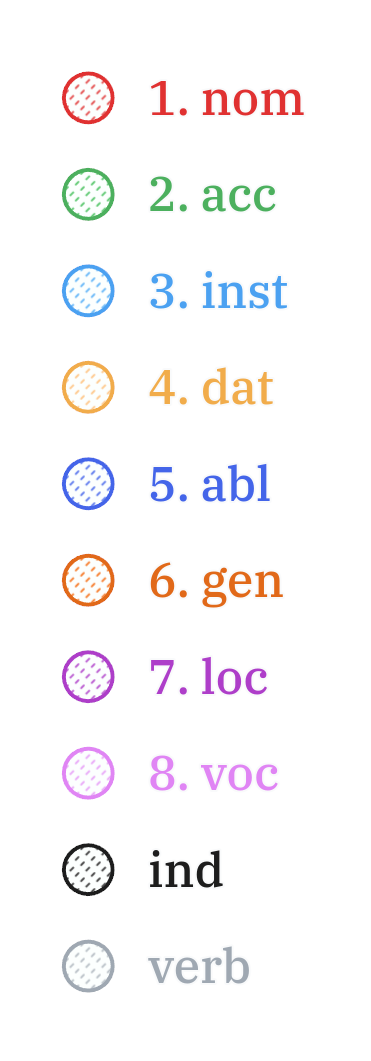
\includegraphics[width=25mm]{./images/cases-legend-white-large.png}%
    }%
  }%
}

\newcommand*\sentenceDiaMsg{\textbf{Exercise:} Draw a sentence analysis diagram below and indicate declensions.}

\newcommand*\sentenceDiaSolution[2][0.4]{%
  \ifanswerkey%
    \hspace*{-\spinemargin}%
    \begin{minipage}{\paperwidth}%
      \centering%
      \includegraphics[scale=#1]{#2}%
    \end{minipage}%
  \else%
    \settototalheight{\@tmp@height}{\includegraphics[scale=#1]{#2}}%
    \begin{minipage}[\@tmp@height]{\linewidth}%
      \sentenceDiaMsg%
    \end{minipage}%
  \fi%
}

\usepackage{cwpuzzle}

\renewcommand\PuzzleCluePre{%
  \begin{minipage}[t]{0.75\linewidth}%
}

\renewcommand\PuzzleClueFont{\fontsize{11}{17}\selectfont}

% \def\PuzzleThickline{\linethickness{2pt}}

\makeatother

\date{\today}
\title{Pali Lessons}
\hypersetup{
 pdfauthor={The Bhikkhu Saṅgha},
 pdftitle={Pali Lessons},
 pdfkeywords={},
 pdfsubject={},
 pdfcreator={Emacs 30.0.50 (Org mode 9.6.1)}, 
 pdflang={En_Gb}}
\begin{document}

\maketitle
\frontmatter

{\centering

{\Huge Pāḷi Lessons}

\bigskip
\href{https://vinaya-class.github.io}{https://vinaya-class.github.io}

{\scshape\small last updated on}\\
\today

}

\bigskip
\tableofcontents*

\mainmatter

\chapter{Lesson 1}
\label{sec:orgd0288c4}
\section{Language Notes}
\label{sec:org333302b}

The \textbf{gender of a noun} is either masculine, feminine or neuter.
Its \textbf{number} is either singular or plural.
Its \textbf{declension} have eight cases, which indicate the subject, object, location, etc.

\textbf{Nouns ending} in \emph{-a} are either masculine or neuter. Nouns ending in \emph{-ā} are feminine.\\[0pt]
Other nouns end in \emph{-i, -ī, -u, -ū}.

\textbf{Word order} in the simplest case is Subject-Object-Verb, but since the case indicates the role of a noun, word order is often altered for emphasis.

\begin{center}
\begin{tabular}{ll}
Sūdo \emph{(nom.sg.)} bhattaṁ \emph{(acc.)} pacati \emph{(3rd.sg.)}. & Dārakā \emph{(nom.sg.)} bhojanīyaṁ \emph{(acc.)} bhuñjanti \emph{(3rd.pl.)}.\\[0pt]
The chef cooks the rice. & The boys eat the food.\\[0pt]
\end{tabular}
\end{center}

The \textbf{subject} and \textbf{verb} must agree in number: \emph{Sakuṇā ākāse uḍḍenti} (Birds fly in the sky).

\begin{center}
\begin{tabular}{lll}
Sakuṇ\textbf{ā} & masc.nom.\textbf{pl.} & Birds\\[0pt]
ākāse / ākāsamhi / ākāsasmiṁ & masc.loc.sg. & in the sky\\[0pt]
uḍḍe\textbf{nti} / uḍḍaya\textbf{nti}. & pr.3.\textbf{pl.} & they fly.\\[0pt]
\end{tabular}
\end{center}

The verb `to be' (is / are) is often implied and dropped from the sentence.

\textbf{An adjective} agrees with the noun it qualifies in gender, number and case. \\[0pt]
Generally, the order is adjective + noun. E.g. \emph{seto asso:} a white horse, \emph{setā assā:} white horses.

\textbf{Adverbs} are indeclinable: \emph{idha} (here), \emph{tattha / tatra} (there), \emph{tato}
(from there), \emph{idāni} (now), \emph{pubbe} (before), \emph{pacchā} (after), etc.

\bigskip

\begin{multicols}{2}

\textbf{Plural / singular} for nominative cases:

\begin{center}
\begin{tabular}{lll}
masc.sg. & -o & devo\\[0pt]
masc.pl. & -ā & devā\\[0pt]
\hline
nt.sg. & -aṁ & rūpaṁ\\[0pt]
nt.pl. & -ā, -āni & rūpāni\\[0pt]
\hline
fem.sg. & -ā & vedanā\\[0pt]
fem.pl. & -ā, -āyo, & vedanāyo\\[0pt]
\end{tabular}
\end{center}

\columnbreak

Personal pronouns in nominative case:

\begin{center}
\begin{tabular}{lll}
 & \textbf{sg.} & \textbf{pl.}\\[0pt]
\textbf{1st} & ahaṁ & amhe, mayaṁ, no\\[0pt]
\textbf{2nd} & tuvaṁ, tvaṁ & tumhe, vo\\[0pt]
\textbf{3rd.masc.} & so, sa & te\\[0pt]
\textbf{3rd.nt.} & taṁ, tad & tāni\\[0pt]
\textbf{3rd.fem.} & sā & tā, tāyo\\[0pt]
\end{tabular}
\end{center}

\emph{sā taṃ bhāsati:} she speaks (to) him/them

\begin{center}
\begin{tabular}{lll}
ta → & \emph{(nom.sg.)} so / taṁ / sā & \emph{(nom.pl.)} te / tāni / tā, tāyo\\[0pt]
 & \emph{(acc.sg.)} taṁ & \emph{(acc.pl.)}  te / tāni / tā, tāyo\\[0pt]
\end{tabular}
\end{center}

\end{multicols}
\bigskip

The 1st and 2nd personal pronouns are gender neutral, the 3rd person pronouns are gendered.

Pronouns take on the person and number of the noun they represent.

A relative sentence begins with a relative clause, followed by a demonstrative:

\begin{center}
\begin{tabular}{llllll}
\emph{yo} & \emph{gilānaṃ} & \emph{upaṭṭhāti} & \emph{so} & \emph{maṃ} & \emph{upaṭṭhāti}\\[0pt]
he who & ill & attends & he & me & attends\\[0pt]
\end{tabular}
\end{center}

\bigskip

\begin{multicols}{2}

\textbf{Negation:} The particle \emph{na} before verbs, shortened as the \emph{a-} prefix for
nouns. \emph{mā + aorist past} is a (present) prohibition.

\emph{avera:} [na + vera] non-hostility \\[0pt]
\emph{Na jānāmi.} I don't know. \\[0pt]
\emph{Mā akāsi!} Don't do!

\columnbreak

\textbf{Questions} begin with interrogatives such as \emph{api, api nu, kiṁ, kahaṁ, kathaṁ}.
\emph{Kiṁ} may be placed at the end of the sentence.

\emph{Api nu gacchasi?} Do you go?\\[0pt]
\emph{Kiṁ nāmo si?} What is your name?\\[0pt]
\emph{Gacchasi kiṁ?} Do you go?

\end{multicols}

\clearpage

\textbf{Declension Table: Masculine Nouns Ending in -a}

\begin{center}
\begin{tabular}{llll}
Case & Singular & Plural & Meaning (sg.)\\[0pt]
\hline
1. Nominative & nar\textbf{o} & nar\textbf{ā} & the man does sth (object)\\[0pt]
2. Accusative & nar\textbf{aṁ} & nar\textbf{e} & sth happens to the man (subject)\\[0pt]
3. Instrumental & nar\textbf{ena} & nar\textbf{ehi} & by, with, through the man\\[0pt]
4. Dative & nar\textbf{āya}, nar\textbf{assa} & nar\textbf{ānaṁ} & to the man, for the man\\[0pt]
5. Ablative & nar\textbf{ā}, nar\textbf{amhā}, nar\textbf{asmā} & nar\textbf{ehi} & from the man\\[0pt]
6. Genitive & nar\textbf{assa} & nar\textbf{ānaṁ} & of the man, the man's\\[0pt]
7. Locative & nar\textbf{e}, nar\textbf{amhi}, nar\textbf{asmiṁ} & nar\textbf{esu} & in, on, at the man\\[0pt]
8. Vocative & nar\textbf{a}, nar\textbf{ā} & nar\textbf{ā} & Hey, man!\\[0pt]
\end{tabular}
\end{center}

This the most common declension, worth memorizing by heart. 87\% of all masculine
nouns are ending in \textbf{-a}, \mbox{97\% of} all neuter nouns are ending in \textbf{-aṁ}, in
addition to adjectives and participles with the same declensions.

\section{Simple Present Tense (-āmi, -asi, -ati)}
\label{sec:orgac2a312}

Actions that are happening at the present moment, occurring regularly, or general truths.

Verbal bases can end in \emph{-a, -ā, -e, -o}.

\bigskip
{\centering\par
\begin{multicols}{2}

Verbal terminations:

\begin{center}
\begin{tabular}{lll}
 & \textbf{sg.} & \textbf{pl.}\\[0pt]
\textbf{1st} & -mi & -ma\\[0pt]
\textbf{2nd} & -si & -tha\\[0pt]
\textbf{3rd} & -ti & -(a)nti\\[0pt]
\end{tabular}
\end{center}

The base is obtained by removing the 3rd.sg. termination \emph{-ti} from the conjugated form.

\columnbreak

Root: \emph{√dhāv} (to run), base: \emph{dhāva}

\begin{center}
\begin{tabular}{lll}
 & \textbf{sg.} & \textbf{pl.}\\[0pt]
\textbf{1st} & dhāvāmi & dhāvāma\\[0pt]
\textbf{2nd} & dhāvasi & dhāvatha\\[0pt]
\textbf{3rd} & dhāvati & dhāvanti\\[0pt]
\end{tabular}
\end{center}

The final \emph{-a} of the base is lengthened before \emph{m}: \emph{dhāvāmi, dhāvāma}.

\end{multicols}
\par}
\bigskip
\begin{multicols}{2}
\setlength{\columnseprule}{0pt}

\begin{center}
\begin{tabular}{ll}
he goes & gacchati\\[0pt]
we go & \fillin{4cm}{gacchāma}\\[0pt]
he comes & āgacchati\\[0pt]
they come & \fillin{4cm}{āgacchanti}\\[0pt]
he walks & carati\\[0pt]
they walk & \fillin{4cm}{caranti}\\[0pt]
he chews & khādati\\[0pt]
you (sg.) chew & \fillin{4cm}{khādasi}\\[0pt]
he eats (enjoys) & bhuñjati\\[0pt]
they eat & \fillin{4cm}{bhuñjanti}\\[0pt]
\end{tabular}
\end{center}

\columnbreak

\begin{center}
\begin{tabular}{ll}
he sees & passati\\[0pt]
you (sg.) see & \fillin{4cm}{passasi}\\[0pt]
he recites & uddisati\\[0pt]
I recite & \fillin{4cm}{uddisāmi}\\[0pt]
he gives (to) & deti\\[0pt]
you (pl.) give (to) & \fillin{4cm}{detha}\\[0pt]
he informs & āroceti\\[0pt]
I inform & \fillin{4cm}{ārocemi}\\[0pt]
he confesses & āvikaroti\\[0pt]
you (sg.) confess & \fillin{4cm}{āvikarosi}\\[0pt]
\end{tabular}
\end{center}

\end{multicols}

\subsection{Present Tense of Irregular Verb √as (to be)}
\label{sec:orga53f6b4}

\begin{center}
\begin{tabular}{lllll}
 & \textbf{sg.} &  & \textbf{pl.} & \\[0pt]
1st & amhi, asmi & I am & amha, amhā, asma & we are\\[0pt]
2nd & asi & you are & attha & you all are\\[0pt]
3rd & atthi & he is & santi & they are\\[0pt]
\end{tabular}
\end{center}

\bigskip

\emph{n'eso'ham'asmi:} [na + eso + ahaṁ + asmi] lit. not this I am

\begin{quote}
\emph{Atthi, bhikkhave, ajātaṁ abhūtaṁ akataṁ asaṅkhataṁ.} (\href{https://suttacentral.net/ud8.3/pli/ms}{Ud 8.3})

\fillin{12cm}{There is, monks, an unborn, unoriginated, uncreated, unfabricated.}
\end{quote}

\subsection{Present Tense of Irregular Verb √hū (to be)}
\label{sec:orgcf5ad0b}

\begin{center}
\begin{tabular}{lllll}
 & \textbf{sg.} &  & \textbf{pl.} & \\[0pt]
1st & homi & I am & homa & we are\\[0pt]
2nd & hosi & you are & hotha & you all are\\[0pt]
3rd & hoti & he is & honti & they are\\[0pt]
\end{tabular}
\end{center}

\section{Declensions (-a)}
\label{sec:org43fe854}
\subsection{Nominative Case: naro -- the man (subject)}
\label{sec:orga1a0b85}

`\textbf{Who} is doing it?' Indicates the \textbf{subject} of a sentence.

\begin{center}
\begin{tabular}{ll}
Naro nisīdati. & \textbf{The man} sits.\\[0pt]
Dārako tiṭṭhati. & \textbf{The boy} stands (tiṭṭhati).\\[0pt]
Mātugāmo uṭṭhahati. & \textbf{The woman} stands up (uṭṭhāti).\\[0pt]
Sīhā na dhāvanti. & \textbf{The lions} are not running.\\[0pt]
Jātā mīyanti. & \textbf{(Those who are) born} (they) die.\\[0pt]
Mallako bhindati. & The cup breaks.\\[0pt]
Abhisatto'va nipatati, vayo.\footnotemark & Like a curse, it falls, \textbf{old age}.\\[0pt]
\end{tabular}
\end{center}\footnotetext[1]{\label{org92b5827}\href{https://suttacentral.net/thag1.118/pli/ms}{Thag 118}}

\subsection{Accusative Case: naraṁ -- the man (object)}
\label{sec:org44532e4}

\textbf{(a)} `\textbf{What} is he eating?' Indicates the \textbf{object} of a sentence.

\renewcommand{\arraystretch}{1.8}

\begin{center}
\begin{tabular}{ll}
I use \textbf{the requisite.} & Parikkhāraṁ paṭisevāmi.\\[0pt]
The birds eat \textbf{the seeds.} (\emph{bīja}) & \fillin{8cm}{Sakuṇā bījāni bhuñjanti.}\\[0pt]
The lion doesn't see \textbf{the dogs.} (\emph{sunakha}) & \fillin{8cm}{Sīho sunakhe na passati.}\\[0pt]
The dogs are barking (\emph{bhussati}) \textbf{at the moon.} (\emph{canda}) & \fillin{8cm}{Sunakhā candaṁ bhussanti.}\\[0pt]
\end{tabular}
\end{center}

\clearpage

\begin{center}
\begin{tabular}{ll}
The disciple (\emph{sāvaka}) eats the lion. & \fillin{8cm}{Sāvako sīhaṁ khādati.}\\[0pt]
The lion eats the disciple. & \fillin{8cm}{Sīho sāvakaṁ khādati.}\\[0pt]
They fill up (\emph{paripūreti}) the ocean (\emph{sāgara}).\footnotemark & \fillin{8cm}{Paripūrenti sāgaraṁ.}\\[0pt]
\end{tabular}
\end{center}\footnotetext[2]{\label{orge63b5ad}Yathā vāri-vahā pūrā\ldots{}}

\normalArrayStrech

\textbf{(b)} `\textbf{Where} is he going to?' Indicates where the subject is \textbf{going to} or \textbf{going along}. \\[0pt]
A.k.a. `the accusative of motion'.

\begin{quote}
\emph{Māluvābījaṁ sālamūle nipatati.} (\href{https://suttacentral.net/mn45/pli/ms}{MN 45})

The māluva-seed (\emph{māluvābīja}) falls \textbf{at the base of sal trees.} (\emph{sālamūla})

\emph{Bhagavā kosalesu cārikaṁ carati\ldots{}} (Ud 5.9)

The Buddha was wandering in the land of the Kosalans\ldots{}
\end{quote}

\renewcommand{\arraystretch}{1.8}

\begin{center}
\begin{tabular}{ll}
The elder is \textbf{going on a walk.} & \fillin{8cm}{Thero cārikaṁ carati.}\\[0pt]
The layman (\emph{upāsaka}) doesn't go \textbf{to the village.} & \fillin{8cm}{Upāsako gāmaṁ na gacchati.}\\[0pt]
We go up to (upasaṅkamati) the layman. & \fillin{8cm}{Upāsakaṁ upasaṅkamāma.}\\[0pt]
The men run \textbf{to the barn.} (\emph{koṭṭhāgāra}) & \fillin{8cm}{Narā koṭṭhāgāraṁ dhāvanti.}\\[0pt]
The birds fly \textbf{to the sal trees.} (\emph{sālarukkha}) & \fillin{8cm}{Sakuṇā sālarukkhe uḍḍenti.}\\[0pt]
We enter (\emph{pavisati}) \textbf{the hut.} (\emph{agāra}) & \fillin{8cm}{Agāraṁ pavisāma.}\\[0pt]
\end{tabular}
\end{center}

\normalArrayStrech

\section{Exercises}
\label{sec:org063e15b}
\subsection{Translate}
\label{sec:org51d9318}

\renewcommand{\arraystretch}{1.8}

\begin{center}
\begin{tabular}{ll}
Saṅgho uposathaṁ karoti. & \fillin{8cm}{The Sangha performs the uposatha.}\\[0pt]
Āpattiṁ āvikaroti. & \fillin{8cm}{He confesses the offense.}\\[0pt]
Suññāgāraṁ pavisāmi. & \fillin{8cm}{I enter the empty hut.}\\[0pt]
Rukkhamūle gacchāma. & \fillin{8cm}{We go to the roots of trees.}\\[0pt]
Cattāro satipaṭṭhānā satta bojjhaṅge paripūrenti.\footnotemark & \fillin{8cm}{The 4 found. of mindf. fulfil the 7 fact. of enligh.  }\\[0pt]
\end{tabular}
\end{center}\footnotetext[3]{\label{org1bd6c3a}\href{https://suttacentral.net/mn118/pli/ms}{MN 118}}

\normalArrayStrech

\subsection{Extra Challenge: Pāli Chat}
\label{sec:org325471a}

\emph{Idha pubbaṇhasamayaṁ Ericeiraṁ piṇḍāya pavisāmi.}

This morning I am entering Ericeira for alms-round.

\emph{Bhante, ayyo āgacchatu, idha nisīdatu.}

Venerable, may the Ven. come and sit here.

\begin{center}
\begin{tabular}{ll}
Good morning! & Supubbaṇho bhante/āvuso.\\[0pt]
Good morning everyone. & Supubbaṇho sabbesaṁ.\\[0pt]
Thank you. & Anumodāmi.\\[0pt]
You're welcome. & Svāgato.\\[0pt]
I (we) must go. & Handa dāni mayaṁ gacchāma.\\[0pt]
Go at your convenience. & Yassadāni tvaṁ kālaṁ maññasī.\\[0pt]
See you tomorrow. & Suve.\\[0pt]
Sorry. & Kāruññaṁ.\\[0pt]
Yes. & Āma, bhante.\\[0pt]
No. & No hetaṁ, bhante.\\[0pt]
Never mind (leave it aside). & Tiṭṭhatu, bhante.\\[0pt]
Excuse me! & Okāsa, bhante.\\[0pt]
Please sit. & Nisīdatha.\\[0pt]
How are you? (I hope you are enduring.) & Kacci te bhante khamanīyaṁ?\\[0pt]
I hope you all are well. & Kacci vo khamanīyaṁ.\\[0pt]
I am alright. & Khamanīyaṁ me, āvuso.\\[0pt]
I am not well. & Na me, bhante, khamanīyaṁ.\\[0pt]
I didn't understand. & Aññāṇamāpādi.\\[0pt]
Why is that? & Taṁ kissa hetu?\\[0pt]
It is very hot / cold today. & Ajjaṁ uṇhakālaṁ / sītakālaṁ.\\[0pt]
Where is the market? & Kattha / Kuhiṁ antarāpaṇaṁ?\\[0pt]
What is your name? & Kinnāmosi?\\[0pt]
My name is \ldots{} & Ahaṁ bhante \ldots{} nāma.\\[0pt]
What is your preceptor's name? & Ko nāma te upajjhāyo?\\[0pt]
My preceptor's name is Ven. \ldots{} & Upajjhāyo me bhante āyasmā \ldots{} nāma.\\[0pt]
aṇha (m.) & day\\[0pt]
sāya (nt.) & night\\[0pt]
samaya (m.) & time; occasion\\[0pt]
supubbaṇha [su + pubba + aṇha] & good morning\\[0pt]
pubbaṇhasamayaṁ & \\[0pt]
sumajjhanhika [su + majjha + anha + ika] & good midday\\[0pt]
majjhanhikasamayaṁ & \\[0pt]
susāyanha [su + sāya + anha] & good evening\\[0pt]
sāyanhasamayaṁ & \\[0pt]
\end{tabular}
\end{center}

(\href{https://suttacentral.net/an3.155/en/sujato}{AN 3.155, Morning})

\chapter{Lesson 2}
\label{sec:orgb5083e6}
\section{Review Exercises}
\label{sec:org656fe82}

\renewcommand{\arraystretch}{1.8}

\begin{center}
\begin{tabular}{ll}
\fillin{8cm}{The elders make an effort.} & Therā viriyaṁ ārabhanti (\emph{begins; undertakes}).\\[0pt]
\fillin{8cm}{They give ear.} & Te sotaṁ odahanti (\emph{applies; gives}).\\[0pt]
The man eats rice. & \fillin{8cm}{Naro bhattaṁ bhuñjati.}\\[0pt]
The men are cooking. & \fillin{8cm}{Narā pacanti.}\\[0pt]
I go up to the man. & \fillin{8cm}{Naraṁ upasaṅkamati.}\\[0pt]
I see the moon. & \fillin{8cm}{Candaṁ passāmi.}\\[0pt]
You (pl.) don't see the dogs. & \fillin{8cm}{Sunakhe na passatha.}\\[0pt]
The boys are running. & \fillin{8cm}{Dārakā dhāvanti.}\\[0pt]
You are sitting here. & \fillin{8cm}{Idha nisīdasi.}\\[0pt]
She comes from there. & \fillin{8cm}{Sā tato āgacchati.}\\[0pt]
We run to the boys. & \fillin{8cm}{Mayaṁ dārake dhāvāma.}\\[0pt]
\end{tabular}
\end{center}

\normalArrayStrech

\section{Declensions (-a)}
\label{sec:org517ceb6}
\subsection{Vocative Case: nara / narā -- Hey, man!}
\label{sec:org215ddd7}

Used when addressing people directly: `Hey layman, come here!' \emph{Ehi upāsak\textbf{a}!}

Vocative singular: all stems ending in \emph{-a, -i, -u} remain unchanged, the final long \emph{-ī, -ū} become short.

Vocative plural: same form as the nominative plural.

\bigskip
{\centering\par
\begin{multicols}{2}

\begin{center}
\begin{tabular}{lll}
stem & sg. & pl.\\[0pt]
\hline
Buddha & Buddha & Buddhā\\[0pt]
muni & muni & munī\\[0pt]
garu & garu & garū\\[0pt]
senānī & senāni & senānī, senānino\\[0pt]
vidū & vidu & vidū\\[0pt]
go & go & gāvo\\[0pt]
\end{tabular}
\end{center}

\columnbreak

Some special vocative forms:

\begin{itemize}
\item \emph{Bho, he:} Hello / hey! (sg.)
\item \emph{Bhavanto} (pl.)
\item \emph{āvuso} (sg.)
\item \emph{bhante} (sg.)
\end{itemize}

\end{multicols}
\par}

\clearpage

\subsection{Imperative Verbs}
\label{sec:org00add3d}

{\centering\par
\begin{multicols}{2}

\begin{center}
\begin{tabular}{lll}
 & \textbf{sg.} & \textbf{pl.}\\[0pt]
\textbf{1st} & -mi & -ma\\[0pt]
\textbf{2nd} & -hi & -tha\\[0pt]
\textbf{3rd} & -tu & -(a)ntu\\[0pt]
\end{tabular}
\end{center}

\columnbreak

\begin{center}
\begin{tabular}{lll}
 & \textbf{sg.} & \textbf{pl.}\\[0pt]
\textbf{1st} & dhāvāmi & dhāvāma\\[0pt]
\textbf{2nd} & dhāva, dhāvāhi & dhāvatha\\[0pt]
\textbf{3rd} & dhāvatu & dhāvantu\\[0pt]
\end{tabular}
\end{center}

\end{multicols}
\par}

Before \emph{-hi}, the final \emph{-a} is lenghened: \emph{dhāvāhi}. The \emph{-hi} may be dropped and the \emph{-ā} shortened: \emph{dhāva}.

The imperative in Pali can express a supplication, a blessing, a command, a gentle advice or a curse.

The particle \emph{mā} is used to express a prohibition.

\begin{center}
\begin{tabular}{ll}
\emph{dhāvāmi} & I may run / May I run / Let me run.\\[0pt]
\emph{dhāvatha} & Run! / You may run / May you run / Let you run.\\[0pt]
\emph{dhāvatu} & He may run / May he run / Let him run.\\[0pt]
\end{tabular}
\end{center}

\renewcommand{\arraystretch}{1.8}

\begin{center}
\begin{tabular}{ll}
Buddho paṭiggaṇhā\textbf{tu} accayantaṃ. & \fillin{8cm}{May the Buddha accept (that) transgression.}\\[0pt]
Phāsu (comfortably) vihara\textbf{tu}! & \fillin{8cm}{Let him live comfortably!}\\[0pt]
Vassasataṁ jīv\textbf{a}! & \fillin{8cm}{May you live 100 years!}\\[0pt]
\textbf{Mā} gaccha! & \fillin{8cm}{Don't go!}\\[0pt]
Suṇātu me bhante saṅgho \ldots{} & \fillin{8cm}{Let the Sangha hear me.}\\[0pt]
Pārisuddhiṁ āyasmanto ārocetha. & \fillin{8cm}{Let the Venerables declare purity.}\\[0pt]
\end{tabular}
\end{center}

\normalArrayStrech

\subsection{Instrumental Case: narena -- with, by, because of the man}
\label{sec:orgd53cd31}

\textbf{`With whom/what? By whom/what? By means of, because of whom/what?'}

\emph{Buddhena}: with the Buddha, by the Buddha, by means of the Buddha, because of the Buddha.

Final \emph{-a} of the stem becomes \emph{-ena}: \emph{Buddha} → \emph{Buddhena}.

In the singular case, to the stems ending in \emph{i, ī, u, ū}, the ending \emph{-nā} is added. The final long vowel of the stem becomes short.

In the plural case, the final long vowel becomes long and \emph{-hi} is added.

\begin{center}
\begin{tabular}{llll}
 &  & \textbf{sg.} & \textbf{pl.}\\[0pt]
ācariya (teacher) & → & ācariyena & ācariyehi\\[0pt]
paṇḍita (sage) & → & \fillin{4cm}{paṇḍitena} & \fillin{4cm}{paṇḍitehi}\\[0pt]
senānī (general) & → & senāninā & senānīhi\\[0pt]
garu (guru) & → & garunā & garūhi\\[0pt]
vidū (seer) & → & vidunā & vidūhi\\[0pt]
viññū (wise man) & → & \fillin{4cm}{viññunā} & \fillin{4cm}{viññūhi}\\[0pt]
\end{tabular}
\end{center}

The particles \textbf{saddhiṁ, saha} used with the instrumental case, expresses the meaning of \textbf{`together with / accompanied by'}.

\textbf{Saddhiṁ} is added after a noun, \textbf{saha} is used as a preposition.

\renewcommand{\arraystretch}{1.8}

\begin{center}
\begin{tabular}{ll}
Buddhena saddhiṁ & together with the Buddha\\[0pt]
\fillin{8cm}{ācariyena / ācariyā saddhiṁ} & together with the teacher\\[0pt]
\fillin{8cm}{viññūhi saddhiṁ} & together with the wise men\\[0pt]
Etena saccena suvatthi hotu.\footnotemark & \fillin{8cm}{By this truth may there be well-being.}\\[0pt]
\fillin{8cm}{Ahaṃ mittena saddhiṃ gāmaṁ gacchāmi.} & I, together with a friend, go to the village.\\[0pt]
\fillin{8cm}{Mātugāmena saddhiṃ cārikaṁ carati.} & He wanders about with a woman. (\emph{mātugāma})\\[0pt]
\end{tabular}
\end{center}\footnotetext[4]{\label{org34f962d}\href{https://suttacentral.net/snp2.1/pli/ms}{Snp 2.1}}

\begin{center}
\begin{tabular}{ll}
Aṭṭhi tacena onaddhaṁ, saha vatthebhi\footnotemark\space sobhati. (MN 82) & \\[0pt]
\fillin{10cm}{A bone covered with skin; it looks beautiful with clothes.} & \\[0pt]
\end{tabular}
\end{center}\footnotetext[5]{\label{orgd655021}The only occurrence of vatth\textbf{ebhi}, normally it's vatth\textbf{ehi}.}

\normalArrayStrech

\begin{itemize}
\item \emph{onaddha}: pp. of onandhati, covered (with); wrapped (with)
\item \emph{vattha}: nt. cloth; clothes; robe
\item \emph{sobhati}: shines (in); looks beautiful (in)
\end{itemize}

\subsection{Dative Case: narāya / narassa -- to the man, for the man}
\label{sec:org6cf1e89}

\textbf{`To whom/what? For whom/what?'}

Singular: final \emph{-a} of the stem becomes \emph{-āya} and \emph{-assa}.

\emph{Buddhāya, Buddhassa}: to or for the Buddha.

\begin{quote}
Saṅgho imaṃ kaṭhinadussaṃ āyasmato Amarassa deti. (\href{https://suttacentral.net/pli-tv-kd7/pli/ms}{Vin. Kd 7})
\end{quote}

To the stems ending in \emph{i, ī, u, ū}, the ending \emph{-no} and \emph{-ssa} are added.

\begin{center}
\begin{tabular}{ll}
Homage to the Buddha. & \fillin{8cm}{Namo Buddhāya / Buddhassa.}\\[0pt]
It leads to Nibbāna. & \fillin{8cm}{Nibbānāya saṁvattati.}\\[0pt]
We eat the almsfood not for fun or indulgence\ldots{} & \fillin{8cm}{Mayaṁ piṇḍapātaṁ bhuñjāma neva davāya, na madāya...}\\[0pt]
\end{tabular}
\end{center}

\begin{quote}
Dasa atthavase:
(1.) saṅghasuṭṭhutāya,
(2.) saṅghaphāsutāya,
(3.) dummaṅkūnaṁ puggalānaṁ \mbox{niggahāya},
(4.) pesalānaṁ bhikkhūnaṁ phāsuvihārāya, \ldots{} (\href{https://suttacentral.net/an10.31/pli/ms}{AN 10.31})
\end{quote}

\subsection{Genitive Case: narassa -- of the man, the man's}
\label{sec:org7d58744}

\textbf{`Of whom/what? Whose?'}

Singular: \emph{-ssa} is added to the final \emph{-a}.

Genitive singular forms of other nouns are the same as the Dative singulars.

\begin{center}
\begin{tabular}{llll}
 &  & Dative & Genitive\\[0pt]
\hline
Buddha & Buddhassa & to/for the Buddha & of the Buddha, the Buddha's\\[0pt]
muni & munino, munissa & to/for the hermit & of the hermit, the hermit's\\[0pt]
senānī & senānino, senānissa & to/for the general & of the general, the general's\\[0pt]
garu & garuno, garussa & to/for the teacher & of the teacher, the teacher's\\[0pt]
vidū & viduno, vidussa & to/for the seer & of the seer, the seer's\\[0pt]
\end{tabular}
\end{center}

The irregular \emph{go} (cow, ox) has two forms: \emph{gavassa, gāvassa} (to/for the cow, of the cow, the cow's).

\begin{quote}
\emph{Na kho pana mayaṁ passāma āyasmato upasenassa kāyassa vā aññathattaṁ indriyānaṁ vā vipariṇāmaṁ.}

But we don't see any impairment in the body or deterioration of Ven. Upasena's faculties. (SN 35.69)
\end{quote}

\renewcommand{\arraystretch}{1.8}

\begin{center}
\begin{tabular}{ll}
\fillin{8cm}{Fire, having rose up, burns down the householder's house.} & Aggi uṭṭhāya (\emph{rose up}) gahapatikassa gehaṁ (\emph{house}) ḍahati (\emph{burns down}).\\[0pt]
\fillin{8cm}{The cooks cook the rice for the householder's servants.} & Sūdehi gahapatino sevakānaṁ odano pacanti.\\[0pt]
\fillin{8cm}{Taken away by thieves, the householder's oxen vanished.} & Corehi haritvā, gahapatino gāvo naṭṭho (\emph{vanished}).\\[0pt]
\fillin{8cm}{The darkness was dispelled by the sun's light.} & Suriyassa ālokena andhakāro (\emph{darkness}) apagato (\emph{lit. gone away}).\\[0pt]
We don't see the change of the body of the man. & \fillin{8cm}{Na passāma manussassa kāyassa vipariṇāmaṁ.}\\[0pt]
By means of the Teaching, men go to the far shore. & \fillin{8cm}{Manussā dhammena pāraṁ gacchanti.}\\[0pt]
The man's oxen were lost / vanished. & \fillin{8cm}{Purisassa goṇo / gāvo naṭṭho.}\\[0pt]
Rice cooked by the cook was eaten (\emph{khādito}) by the beggar's (\emph{yācaka}) dog. & \fillin{8cm}{Sūdena pacito odano yācakassa sunakhena khādito.}\\[0pt]
\end{tabular}
\end{center}

\normalArrayStrech

\section{Optative or Potential Verbs: May / Should (-eyya)}
\label{sec:org8c8a553}

{\centering\par
\begin{multicols}{2}

Verbal terminations:

\begin{center}
\begin{tabular}{lll}
 & \textbf{sg.} & \textbf{pl.}\\[0pt]
\textbf{1st} & -eyyāmi, -emi & -eyyāma, -ema\\[0pt]
\textbf{2nd} & -eyyāsi, -esi & -eyyātha, -etha\\[0pt]
\textbf{3rd} & -eyya, -e & -eyyuṁ\\[0pt]
\end{tabular}
\end{center}

\columnbreak

Root: \emph{√dhāv} (to run), base: \emph{dhāva}

\begin{center}
\begin{tabular}{lll}
 & \textbf{sg.} & \textbf{pl.}\\[0pt]
\textbf{1st} & dhāveyyāmi, dhāvemi & dhāveyyāma, dhāvema\\[0pt]
\textbf{2nd} & dhāveyyāsi, dhāvesi & dhāveyyātha, dhāvetha\\[0pt]
\textbf{3rd} & dhāveyya, dhāve & dhāveyyuṁ\\[0pt]
\end{tabular}
\end{center}

\end{multicols}
\par}

Irregular forms:

{\centering\par
\begin{multicols}{2}

\emph{√as} (to be), \emph{atthi}

\begin{center}
\begin{tabular}{lll}
 & \textbf{sg.} & \textbf{pl.}\\[0pt]
\textbf{1st} & siyaṁ, assaṁ & assāma\\[0pt]
\textbf{2nd} & siyā, assa & assatha\\[0pt]
\textbf{3rd} & siyā, assa & siyuṁ, assu, siyaṁsu\\[0pt]
\end{tabular}
\end{center}

\columnbreak

\emph{√kar} (to do, make, work), \emph{karo}

\begin{center}
\begin{tabular}{lll}
 & \textbf{sg.} & \textbf{pl.}\\[0pt]
\textbf{1st} & kareyyāmi, kayirāmi & kareyyāma, kayirāma\\[0pt]
\textbf{2nd} & kareyyāsi, kayirāsi & kareyyātha, kayirātha\\[0pt]
\textbf{3rd} & kareyya, kayirā, kare & kareyyuṁ, kayiruṁ\\[0pt]
\end{tabular}
\end{center}

\end{multicols}
\par}

The optative generally indicates that the situation is hypothetical. It is often used to imply sense of `if'.

\begin{quote}
\emph{Yadā tumhe, bhaddiya, attanāva jāneyyātha\ldots{}} (\href{https://suttacentral.net/an4.193/pli/ms}{AN 4.193})

\fillin{10cm}{When (if) you, Bhaddiya, know this by yourself...}
\end{quote}

The optative cam imply a polite imperative, `it would be good if you\ldots{}'

\begin{quote}
\emph{Ime dhammā kusalā \ldots{} hitāya sukhāya saṁvattantī'ti,}

\fillin{10cm}{These things are wholesome ... lead to long-term happiness,}

\emph{atha tumhe, kālāmā, upasampajja (undertaking, attaining) vihareyyātha.} (\href{https://suttacentral.net/an3.65/pli/ms}{AN 3.65})

\fillin{10cm}{then, Kālāmas, you should undertake them and abide in them...}
\end{quote}

\subsection{Optative of √as (to be) has two forms}
\label{sec:org42ddcff}

\begin{center}
\begin{tabular}{lllll}
1st & assaṁ & I could be & assāma & we could be\\[0pt]
 & siyaṁ &  & -- & \\[0pt]
\hline
2nd & assa & you could be & assatha & you could be\\[0pt]
 & siyā &  & -- & \\[0pt]
\hline
3rd & assa & he could be & assu & they could be\\[0pt]
 & siyā &  & siyaṁsu, siyuṁ & \\[0pt]
\end{tabular}
\end{center}

\begin{quote}
\emph{Aho vata mayaṁ na maraṇadhammā assāma!} (DN 22)

If only we could not be of the nature to die!
\end{quote}

\section{Future Passive Participle: Should Be Done (-tabba)}
\label{sec:org8236fb5}

A.k.a. the gerundive form, formed by adding \emph{-tabba, -anīya, -ya} either to the
present active base or to the verbal root. In the root, \emph{i → e} and \emph{u → o}.
The final \emph{-ā} of the root is changed into \emph{e} before \emph{-ya}, and \emph{y} is reduplicated.

\bigskip
{\centering\par
\begin{multicols}{2}

\begin{center}
\begin{tabular}{lll}
√dā & dātabba, deyya & should be given\\[0pt]
√nī & nettabba & should be led\\[0pt]
√su & sotabba & should be listened to\\[0pt]
dese & desetabba & should be expounded\\[0pt]
\end{tabular}
\end{center}

\columnbreak

\begin{center}
\begin{tabular}{lll}
√kar & kātabba, karaṇīya & should be done\\[0pt]
√ñā & ñātabba, ñeyya & should be known\\[0pt]
√pā & peyya & should be drunk\\[0pt]
kiṇā & kīṇeyya & should be bought\\[0pt]
\end{tabular}
\end{center}

\end{multicols}
\par}

\section{Exercises}
\label{sec:org04b6444}
\subsection{Translate}
\label{sec:org25d37cd}

\renewcommand{\arraystretch}{1.8}

\begin{center}
\begin{tabular}{ll}
TODO & \fillin{8cm}{TODO}\\[0pt]
 & \fillin{8cm}{}\\[0pt]
 & \fillin{8cm}{}\\[0pt]
 & \fillin{8cm}{}\\[0pt]
 & \fillin{8cm}{}\\[0pt]
 & \fillin{8cm}{}\\[0pt]
\end{tabular}
\end{center}

\normalArrayStrech

\clearpage

\subsection{Readings}
\label{sec:org61d58ba}

Kusalañca hidaṁ, bhikkhave, bhāvitaṁ ahitāya dukkhāya saṁvatteyya, nāhaṁ evaṁ vadeyyaṁ: `kusalaṁ, bhikkhave, bhāvethā'ti. (\href{https://suttacentral.net/an2.11-20/pli/ms}{AN 2.11-20})

(bhāvetha + iti → bhāvethā'ti, a + i → ā)

\noindent\rule{\textwidth}{0.5pt}

Yo pana bhikkhu sañcicca pāṇaṁ jīvitā voropeyya, pācittiyaṁ. (\href{https://suttacentral.net/pli-tv-bu-vb-pc61/pli/ms}{Pc 61})

Sikkhamānena, bhikkhave, bhikkhunā aññātabbaṁ paripucchitabbaṁ paripañhitabbaṁ. (Pc 71)

Yo pana bhikkhu otiṇṇo vipariṇatena cittena mātugāmena saddhiṁ kāyasaṁsaggaṁ samāpajjeyya \ldots{} (Sg 2)

\begin{itemize}
\item \emph{vipariṇamati}: he changes, alters, distorts
\item \emph{vipariṇata}: changed, altered, distorted (pp. vipariṇamati)
\item \emph{viparinatena}: with/by a changed, altered, distorted state
\end{itemize}

Yo pana bhikkhu bhikkhussa kupito anattamano pahāraṁ dadeyya, pācittiyaṁ. (Pc 74)

Agilānena bhikkhunā eko āvasathapiṇḍo bhuñjitabbo. Tato ce uttariṁ bhuñjeyya, pācittiyaṁ. (Pc 31)

\noindent\rule{\textwidth}{0.5pt}

Suṇātu me bhante saṅgho. \\[0pt]
Ajj'uposatho paṇṇaraso. \\[0pt]
Yadi saṅghassa pattakallaṁ, \\[0pt]
saṅgho uposathaṁ kareyya, \\[0pt]
pāṭimokkhaṁ uddisseyya.

Kiṁ saṅghassa pubba-kiccaṁ? \\[0pt]
Pārisuddhiṁ āyasmanto ārocetha. \\[0pt]
Pāṭimokkhaṁ uddisissāmi. \\[0pt]
Taṁ sabbeva santā sādhukaṁ \\[0pt]
suṇoma manasikaroma. \\[0pt]
Yassa siyā āpatti, so āvikareyya. \\[0pt]
Asantiyā [na + santi + yā] āpattiyā tuṇhī bhāvitabbaṁ. \\[0pt]
Tuṇhī-bhāvena kho pan'āyasmante \\[0pt]
pārisuddhā ti vedissāmi.

(Nidāna)

\subsection{Extra Challenge: Crossword}
\label{sec:org8e608cb}

\begin{Puzzle}{13}{9}%
\documentclass[10pt, a4paper]{article}

\makeatletter

\usepackage{graphicx}
\graphicspath{{./assets/}}

\usepackage{multicol}

\usepackage{geometry}
\geometry{
  a4paper,
  top = 10mm,
  bottom = 20mm,
  hmargin = 20mm,
}

\usepackage{fontspec}
\setmainfont{Linux Libertine}

\def\BOOK@fontSizePt{10}
\def\BOOK@lineHeightPt{18}

\renewcommand{\normalsize}{%
  \@setfontsize\normalsize\BOOK@fontSizePt\BOOK@lineHeightPt
  \abovedisplayskip 11\p@ \@plus3\p@ \@minus6\p@
  \abovedisplayshortskip \z@ \@plus3\p@
  \belowdisplayshortskip 6.5\p@ \@plus3.5\p@ \@minus3\p@
  \belowdisplayskip \abovedisplayskip
  %\color{textbody}
  \let\@listi\@listI}
\normalsize

\usepackage{cwpuzzle}

\renewcommand\PuzzleCluePre{%
  \begin{minipage}[t]{0.75\linewidth}%
}

\renewcommand\PuzzleClueFont{\fontsize{10}{17}\selectfont}

% \def\PuzzleThickline{\linethickness{2pt}}

\pagestyle{empty}

\makeatother

\begin{document}

\begin{Puzzle}{13}{9}%
\documentclass[10pt, a4paper]{article}

\makeatletter

\usepackage{graphicx}
\graphicspath{{./assets/}}

\usepackage{multicol}

\usepackage{geometry}
\geometry{
  a4paper,
  top = 10mm,
  bottom = 20mm,
  hmargin = 20mm,
}

\usepackage{fontspec}
\setmainfont{Linux Libertine}

\def\BOOK@fontSizePt{10}
\def\BOOK@lineHeightPt{18}

\renewcommand{\normalsize}{%
  \@setfontsize\normalsize\BOOK@fontSizePt\BOOK@lineHeightPt
  \abovedisplayskip 11\p@ \@plus3\p@ \@minus6\p@
  \abovedisplayshortskip \z@ \@plus3\p@
  \belowdisplayshortskip 6.5\p@ \@plus3.5\p@ \@minus3\p@
  \belowdisplayskip \abovedisplayskip
  %\color{textbody}
  \let\@listi\@listI}
\normalsize

\usepackage{cwpuzzle}

\renewcommand\PuzzleCluePre{%
  \begin{minipage}[t]{0.75\linewidth}%
}

\renewcommand\PuzzleClueFont{\fontsize{10}{17}\selectfont}

% \def\PuzzleThickline{\linethickness{2pt}}

\pagestyle{empty}

\makeatother

\begin{document}

\begin{Puzzle}{13}{9}%
\documentclass[10pt, a4paper]{article}

\makeatletter

\usepackage{graphicx}
\graphicspath{{./assets/}}

\usepackage{multicol}

\usepackage{geometry}
\geometry{
  a4paper,
  top = 10mm,
  bottom = 20mm,
  hmargin = 20mm,
}

\usepackage{fontspec}
\setmainfont{Linux Libertine}

\def\BOOK@fontSizePt{10}
\def\BOOK@lineHeightPt{18}

\renewcommand{\normalsize}{%
  \@setfontsize\normalsize\BOOK@fontSizePt\BOOK@lineHeightPt
  \abovedisplayskip 11\p@ \@plus3\p@ \@minus6\p@
  \abovedisplayshortskip \z@ \@plus3\p@
  \belowdisplayshortskip 6.5\p@ \@plus3.5\p@ \@minus3\p@
  \belowdisplayskip \abovedisplayskip
  %\color{textbody}
  \let\@listi\@listI}
\normalsize

\usepackage{cwpuzzle}

\renewcommand\PuzzleCluePre{%
  \begin{minipage}[t]{0.75\linewidth}%
}

\renewcommand\PuzzleClueFont{\fontsize{10}{17}\selectfont}

% \def\PuzzleThickline{\linethickness{2pt}}

\pagestyle{empty}

\makeatother

\begin{document}

\begin{Puzzle}{13}{9}%
\input{./assets/cw-01.txt}
\end{Puzzle}

\vspace*{-\baselineskip}

\begin{multicols}{2}

\begin{PuzzleClues}{\textbf{Tiriyato}}
  \mbox{}\\
  \Clue{1}{putta}{mātāya dāraka}\\
  \Clue{2}{pīti}{TODO}\\
  \Clue{4}{kuṭi}{bhikkhussa vihāraṁ}\\
  \Clue{5}{cīvara}{bhikkhussa dussaṁ}\\
  \Clue{7}{tapati}{kilesaṁ jhāyati}\\
  \Clue{10}{aratī}{TODO}\\
  \Clue{11}{gimha}{TODO}\\
  \Clue{13}{gāviṁ}{TODO}\\
  \Clue{14}{kataññū}{vedeti (having received)}\\
  \Clue{15}{rahāyati}{TODO}\\
  \Clue{16}{ādi}{TODO}
\end{PuzzleClues}

\columnbreak

\begin{PuzzleClues}{\textbf{Dīghaso}}
  \mbox{}\\
  \Clue{1}{pacati}{sūdassa kammaṁ}\\
  \Clue{2}{pivati}{TODO}\\
  \Clue{3}{tatra}{TODO}\\
  \Clue{4}{kattikā}{TODO}\\
  \Clue{6}{vidū}{paṇḍito}\\
  \Clue{8}{patta}{TODO}\\
  \Clue{9}{aggi}{TODO}\\
  \Clue{10}{ahiri}{TODO}\\
  \Clue{12}{rūpa}{TODO}
\end{PuzzleClues}

\end{multicols}

\clearpage

\PuzzleSolution[true]

\begin{Puzzle}{13}{9}%
\input{./assets/cw-01.txt}
\end{Puzzle}

\end{document}

\end{Puzzle}

\vspace*{-\baselineskip}

\begin{multicols}{2}

\begin{PuzzleClues}{\textbf{Tiriyato}}
  \mbox{}\\
  \Clue{1}{putta}{mātāya dāraka}\\
  \Clue{2}{pīti}{TODO}\\
  \Clue{4}{kuṭi}{bhikkhussa vihāraṁ}\\
  \Clue{5}{cīvara}{bhikkhussa dussaṁ}\\
  \Clue{7}{tapati}{kilesaṁ jhāyati}\\
  \Clue{10}{aratī}{TODO}\\
  \Clue{11}{gimha}{TODO}\\
  \Clue{13}{gāviṁ}{TODO}\\
  \Clue{14}{kataññū}{vedeti (having received)}\\
  \Clue{15}{rahāyati}{TODO}\\
  \Clue{16}{ādi}{TODO}
\end{PuzzleClues}

\columnbreak

\begin{PuzzleClues}{\textbf{Dīghaso}}
  \mbox{}\\
  \Clue{1}{pacati}{sūdassa kammaṁ}\\
  \Clue{2}{pivati}{TODO}\\
  \Clue{3}{tatra}{TODO}\\
  \Clue{4}{kattikā}{TODO}\\
  \Clue{6}{vidū}{paṇḍito}\\
  \Clue{8}{patta}{TODO}\\
  \Clue{9}{aggi}{TODO}\\
  \Clue{10}{ahiri}{TODO}\\
  \Clue{12}{rūpa}{TODO}
\end{PuzzleClues}

\end{multicols}

\clearpage

\PuzzleSolution[true]

\begin{Puzzle}{13}{9}%
\documentclass[10pt, a4paper]{article}

\makeatletter

\usepackage{graphicx}
\graphicspath{{./assets/}}

\usepackage{multicol}

\usepackage{geometry}
\geometry{
  a4paper,
  top = 10mm,
  bottom = 20mm,
  hmargin = 20mm,
}

\usepackage{fontspec}
\setmainfont{Linux Libertine}

\def\BOOK@fontSizePt{10}
\def\BOOK@lineHeightPt{18}

\renewcommand{\normalsize}{%
  \@setfontsize\normalsize\BOOK@fontSizePt\BOOK@lineHeightPt
  \abovedisplayskip 11\p@ \@plus3\p@ \@minus6\p@
  \abovedisplayshortskip \z@ \@plus3\p@
  \belowdisplayshortskip 6.5\p@ \@plus3.5\p@ \@minus3\p@
  \belowdisplayskip \abovedisplayskip
  %\color{textbody}
  \let\@listi\@listI}
\normalsize

\usepackage{cwpuzzle}

\renewcommand\PuzzleCluePre{%
  \begin{minipage}[t]{0.75\linewidth}%
}

\renewcommand\PuzzleClueFont{\fontsize{10}{17}\selectfont}

% \def\PuzzleThickline{\linethickness{2pt}}

\pagestyle{empty}

\makeatother

\begin{document}

\begin{Puzzle}{13}{9}%
\input{./assets/cw-01.txt}
\end{Puzzle}

\vspace*{-\baselineskip}

\begin{multicols}{2}

\begin{PuzzleClues}{\textbf{Tiriyato}}
  \mbox{}\\
  \Clue{1}{putta}{mātāya dāraka}\\
  \Clue{2}{pīti}{TODO}\\
  \Clue{4}{kuṭi}{bhikkhussa vihāraṁ}\\
  \Clue{5}{cīvara}{bhikkhussa dussaṁ}\\
  \Clue{7}{tapati}{kilesaṁ jhāyati}\\
  \Clue{10}{aratī}{TODO}\\
  \Clue{11}{gimha}{TODO}\\
  \Clue{13}{gāviṁ}{TODO}\\
  \Clue{14}{kataññū}{vedeti (having received)}\\
  \Clue{15}{rahāyati}{TODO}\\
  \Clue{16}{ādi}{TODO}
\end{PuzzleClues}

\columnbreak

\begin{PuzzleClues}{\textbf{Dīghaso}}
  \mbox{}\\
  \Clue{1}{pacati}{sūdassa kammaṁ}\\
  \Clue{2}{pivati}{TODO}\\
  \Clue{3}{tatra}{TODO}\\
  \Clue{4}{kattikā}{TODO}\\
  \Clue{6}{vidū}{paṇḍito}\\
  \Clue{8}{patta}{TODO}\\
  \Clue{9}{aggi}{TODO}\\
  \Clue{10}{ahiri}{TODO}\\
  \Clue{12}{rūpa}{TODO}
\end{PuzzleClues}

\end{multicols}

\clearpage

\PuzzleSolution[true]

\begin{Puzzle}{13}{9}%
\input{./assets/cw-01.txt}
\end{Puzzle}

\end{document}

\end{Puzzle}

\end{document}

\end{Puzzle}

\vspace*{-\baselineskip}

\begin{multicols}{2}

\begin{PuzzleClues}{\textbf{Tiriyato}}
  \mbox{}\\
  \Clue{1}{putta}{mātāya dāraka}\\
  \Clue{2}{pīti}{TODO}\\
  \Clue{4}{kuṭi}{bhikkhussa vihāraṁ}\\
  \Clue{5}{cīvara}{bhikkhussa dussaṁ}\\
  \Clue{7}{tapati}{kilesaṁ jhāyati}\\
  \Clue{10}{aratī}{TODO}\\
  \Clue{11}{gimha}{TODO}\\
  \Clue{13}{gāviṁ}{TODO}\\
  \Clue{14}{kataññū}{vedeti (having received)}\\
  \Clue{15}{rahāyati}{TODO}\\
  \Clue{16}{ādi}{TODO}
\end{PuzzleClues}

\columnbreak

\begin{PuzzleClues}{\textbf{Dīghaso}}
  \mbox{}\\
  \Clue{1}{pacati}{sūdassa kammaṁ}\\
  \Clue{2}{pivati}{TODO}\\
  \Clue{3}{tatra}{TODO}\\
  \Clue{4}{kattikā}{TODO}\\
  \Clue{6}{vidū}{paṇḍito}\\
  \Clue{8}{patta}{TODO}\\
  \Clue{9}{aggi}{TODO}\\
  \Clue{10}{ahiri}{TODO}\\
  \Clue{12}{rūpa}{TODO}
\end{PuzzleClues}

\end{multicols}

\clearpage

\PuzzleSolution[true]

\begin{Puzzle}{13}{9}%
\documentclass[10pt, a4paper]{article}

\makeatletter

\usepackage{graphicx}
\graphicspath{{./assets/}}

\usepackage{multicol}

\usepackage{geometry}
\geometry{
  a4paper,
  top = 10mm,
  bottom = 20mm,
  hmargin = 20mm,
}

\usepackage{fontspec}
\setmainfont{Linux Libertine}

\def\BOOK@fontSizePt{10}
\def\BOOK@lineHeightPt{18}

\renewcommand{\normalsize}{%
  \@setfontsize\normalsize\BOOK@fontSizePt\BOOK@lineHeightPt
  \abovedisplayskip 11\p@ \@plus3\p@ \@minus6\p@
  \abovedisplayshortskip \z@ \@plus3\p@
  \belowdisplayshortskip 6.5\p@ \@plus3.5\p@ \@minus3\p@
  \belowdisplayskip \abovedisplayskip
  %\color{textbody}
  \let\@listi\@listI}
\normalsize

\usepackage{cwpuzzle}

\renewcommand\PuzzleCluePre{%
  \begin{minipage}[t]{0.75\linewidth}%
}

\renewcommand\PuzzleClueFont{\fontsize{10}{17}\selectfont}

% \def\PuzzleThickline{\linethickness{2pt}}

\pagestyle{empty}

\makeatother

\begin{document}

\begin{Puzzle}{13}{9}%
\documentclass[10pt, a4paper]{article}

\makeatletter

\usepackage{graphicx}
\graphicspath{{./assets/}}

\usepackage{multicol}

\usepackage{geometry}
\geometry{
  a4paper,
  top = 10mm,
  bottom = 20mm,
  hmargin = 20mm,
}

\usepackage{fontspec}
\setmainfont{Linux Libertine}

\def\BOOK@fontSizePt{10}
\def\BOOK@lineHeightPt{18}

\renewcommand{\normalsize}{%
  \@setfontsize\normalsize\BOOK@fontSizePt\BOOK@lineHeightPt
  \abovedisplayskip 11\p@ \@plus3\p@ \@minus6\p@
  \abovedisplayshortskip \z@ \@plus3\p@
  \belowdisplayshortskip 6.5\p@ \@plus3.5\p@ \@minus3\p@
  \belowdisplayskip \abovedisplayskip
  %\color{textbody}
  \let\@listi\@listI}
\normalsize

\usepackage{cwpuzzle}

\renewcommand\PuzzleCluePre{%
  \begin{minipage}[t]{0.75\linewidth}%
}

\renewcommand\PuzzleClueFont{\fontsize{10}{17}\selectfont}

% \def\PuzzleThickline{\linethickness{2pt}}

\pagestyle{empty}

\makeatother

\begin{document}

\begin{Puzzle}{13}{9}%
\input{./assets/cw-01.txt}
\end{Puzzle}

\vspace*{-\baselineskip}

\begin{multicols}{2}

\begin{PuzzleClues}{\textbf{Tiriyato}}
  \mbox{}\\
  \Clue{1}{putta}{mātāya dāraka}\\
  \Clue{2}{pīti}{TODO}\\
  \Clue{4}{kuṭi}{bhikkhussa vihāraṁ}\\
  \Clue{5}{cīvara}{bhikkhussa dussaṁ}\\
  \Clue{7}{tapati}{kilesaṁ jhāyati}\\
  \Clue{10}{aratī}{TODO}\\
  \Clue{11}{gimha}{TODO}\\
  \Clue{13}{gāviṁ}{TODO}\\
  \Clue{14}{kataññū}{vedeti (having received)}\\
  \Clue{15}{rahāyati}{TODO}\\
  \Clue{16}{ādi}{TODO}
\end{PuzzleClues}

\columnbreak

\begin{PuzzleClues}{\textbf{Dīghaso}}
  \mbox{}\\
  \Clue{1}{pacati}{sūdassa kammaṁ}\\
  \Clue{2}{pivati}{TODO}\\
  \Clue{3}{tatra}{TODO}\\
  \Clue{4}{kattikā}{TODO}\\
  \Clue{6}{vidū}{paṇḍito}\\
  \Clue{8}{patta}{TODO}\\
  \Clue{9}{aggi}{TODO}\\
  \Clue{10}{ahiri}{TODO}\\
  \Clue{12}{rūpa}{TODO}
\end{PuzzleClues}

\end{multicols}

\clearpage

\PuzzleSolution[true]

\begin{Puzzle}{13}{9}%
\input{./assets/cw-01.txt}
\end{Puzzle}

\end{document}

\end{Puzzle}

\vspace*{-\baselineskip}

\begin{multicols}{2}

\begin{PuzzleClues}{\textbf{Tiriyato}}
  \mbox{}\\
  \Clue{1}{putta}{mātāya dāraka}\\
  \Clue{2}{pīti}{TODO}\\
  \Clue{4}{kuṭi}{bhikkhussa vihāraṁ}\\
  \Clue{5}{cīvara}{bhikkhussa dussaṁ}\\
  \Clue{7}{tapati}{kilesaṁ jhāyati}\\
  \Clue{10}{aratī}{TODO}\\
  \Clue{11}{gimha}{TODO}\\
  \Clue{13}{gāviṁ}{TODO}\\
  \Clue{14}{kataññū}{vedeti (having received)}\\
  \Clue{15}{rahāyati}{TODO}\\
  \Clue{16}{ādi}{TODO}
\end{PuzzleClues}

\columnbreak

\begin{PuzzleClues}{\textbf{Dīghaso}}
  \mbox{}\\
  \Clue{1}{pacati}{sūdassa kammaṁ}\\
  \Clue{2}{pivati}{TODO}\\
  \Clue{3}{tatra}{TODO}\\
  \Clue{4}{kattikā}{TODO}\\
  \Clue{6}{vidū}{paṇḍito}\\
  \Clue{8}{patta}{TODO}\\
  \Clue{9}{aggi}{TODO}\\
  \Clue{10}{ahiri}{TODO}\\
  \Clue{12}{rūpa}{TODO}
\end{PuzzleClues}

\end{multicols}

\clearpage

\PuzzleSolution[true]

\begin{Puzzle}{13}{9}%
\documentclass[10pt, a4paper]{article}

\makeatletter

\usepackage{graphicx}
\graphicspath{{./assets/}}

\usepackage{multicol}

\usepackage{geometry}
\geometry{
  a4paper,
  top = 10mm,
  bottom = 20mm,
  hmargin = 20mm,
}

\usepackage{fontspec}
\setmainfont{Linux Libertine}

\def\BOOK@fontSizePt{10}
\def\BOOK@lineHeightPt{18}

\renewcommand{\normalsize}{%
  \@setfontsize\normalsize\BOOK@fontSizePt\BOOK@lineHeightPt
  \abovedisplayskip 11\p@ \@plus3\p@ \@minus6\p@
  \abovedisplayshortskip \z@ \@plus3\p@
  \belowdisplayshortskip 6.5\p@ \@plus3.5\p@ \@minus3\p@
  \belowdisplayskip \abovedisplayskip
  %\color{textbody}
  \let\@listi\@listI}
\normalsize

\usepackage{cwpuzzle}

\renewcommand\PuzzleCluePre{%
  \begin{minipage}[t]{0.75\linewidth}%
}

\renewcommand\PuzzleClueFont{\fontsize{10}{17}\selectfont}

% \def\PuzzleThickline{\linethickness{2pt}}

\pagestyle{empty}

\makeatother

\begin{document}

\begin{Puzzle}{13}{9}%
\input{./assets/cw-01.txt}
\end{Puzzle}

\vspace*{-\baselineskip}

\begin{multicols}{2}

\begin{PuzzleClues}{\textbf{Tiriyato}}
  \mbox{}\\
  \Clue{1}{putta}{mātāya dāraka}\\
  \Clue{2}{pīti}{TODO}\\
  \Clue{4}{kuṭi}{bhikkhussa vihāraṁ}\\
  \Clue{5}{cīvara}{bhikkhussa dussaṁ}\\
  \Clue{7}{tapati}{kilesaṁ jhāyati}\\
  \Clue{10}{aratī}{TODO}\\
  \Clue{11}{gimha}{TODO}\\
  \Clue{13}{gāviṁ}{TODO}\\
  \Clue{14}{kataññū}{vedeti (having received)}\\
  \Clue{15}{rahāyati}{TODO}\\
  \Clue{16}{ādi}{TODO}
\end{PuzzleClues}

\columnbreak

\begin{PuzzleClues}{\textbf{Dīghaso}}
  \mbox{}\\
  \Clue{1}{pacati}{sūdassa kammaṁ}\\
  \Clue{2}{pivati}{TODO}\\
  \Clue{3}{tatra}{TODO}\\
  \Clue{4}{kattikā}{TODO}\\
  \Clue{6}{vidū}{paṇḍito}\\
  \Clue{8}{patta}{TODO}\\
  \Clue{9}{aggi}{TODO}\\
  \Clue{10}{ahiri}{TODO}\\
  \Clue{12}{rūpa}{TODO}
\end{PuzzleClues}

\end{multicols}

\clearpage

\PuzzleSolution[true]

\begin{Puzzle}{13}{9}%
\input{./assets/cw-01.txt}
\end{Puzzle}

\end{document}

\end{Puzzle}

\end{document}

\end{Puzzle}

\end{document}

\end{Puzzle}

\vspace*{\baselineskip}

\begin{multicols}{2}

\begin{PuzzleClues}{\textbf{Tiriyato}}
  \mbox{}\\
  \Clue{1}{putta}{mātuyā dāraka}\\
  \Clue{2}{pīti}{pāmojja; sukha}\\
  \Clue{4}{kuṭi}{bhikkhussa vihāraṁ}\\
  \Clue{5}{cīvara}{bhikkhussa dussaṁ}\\
  \Clue{7}{tapati}{kilesaṁ jhāyati}\\
  \Clue{10}{aratī}{so na vedeti samito; eko māradhītaro}\\
  \Clue{11}{gimha}{vassassa eko utu}\\
  \Clue{14}{gāviṁ}{Kassako \ldots{} gāmaṁ nayati.}\\
  \Clue{15}{kataññū}{Piṇḍaṁ paṭiggahetvā so vedeti}\\
  \Clue{16}{rahāyati}{vivekaṁ icchati; ekako viharati}\\
  \Clue{17}{ādi}{\ldots{}, majjima, pariyosāna}
\end{PuzzleClues}

\columnbreak

\begin{PuzzleClues}{\textbf{Dīghaso}}
  \mbox{}\\
  \Clue{1}{pacati}{sūdassa kammaṁ}\\
  \Clue{2}{pivati}{bhuñjitvā naro pānīyaṁ \ldots{}}\\
  \Clue{3}{tatra}{nocidha}\\
  \Clue{4}{kattikā}{gimhānaṁ pacchimaṁ māsaṁ}\\
  \Clue{6}{vidū}{viññū; paṇḍito}\\
  \Clue{8}{patta}{tato bhikkhu bhuñjati}\\
  \Clue{9}{aggi}{gahapatikassa gehaṁ vināseti}\\
  \Clue{12}{hiri}{eko lokapālakadhammo}\\
  \Clue{13}{rūpa}{eko khandho}
\end{PuzzleClues}

\end{multicols}


\ifanswerkey

\vspace*{\baselineskip}

\PuzzleSolution[true]

\begin{Puzzle}{13}{9}%
\documentclass[10pt, a4paper]{article}

\makeatletter

\usepackage{graphicx}
\graphicspath{{./assets/}}

\usepackage{multicol}

\usepackage{geometry}
\geometry{
  a4paper,
  top = 10mm,
  bottom = 20mm,
  hmargin = 20mm,
}

\usepackage{fontspec}
\setmainfont{Linux Libertine}

\def\BOOK@fontSizePt{10}
\def\BOOK@lineHeightPt{18}

\renewcommand{\normalsize}{%
  \@setfontsize\normalsize\BOOK@fontSizePt\BOOK@lineHeightPt
  \abovedisplayskip 11\p@ \@plus3\p@ \@minus6\p@
  \abovedisplayshortskip \z@ \@plus3\p@
  \belowdisplayshortskip 6.5\p@ \@plus3.5\p@ \@minus3\p@
  \belowdisplayskip \abovedisplayskip
  %\color{textbody}
  \let\@listi\@listI}
\normalsize

\usepackage{cwpuzzle}

\renewcommand\PuzzleCluePre{%
  \begin{minipage}[t]{0.75\linewidth}%
}

\renewcommand\PuzzleClueFont{\fontsize{10}{17}\selectfont}

% \def\PuzzleThickline{\linethickness{2pt}}

\pagestyle{empty}

\makeatother

\begin{document}

\begin{Puzzle}{13}{9}%
\documentclass[10pt, a4paper]{article}

\makeatletter

\usepackage{graphicx}
\graphicspath{{./assets/}}

\usepackage{multicol}

\usepackage{geometry}
\geometry{
  a4paper,
  top = 10mm,
  bottom = 20mm,
  hmargin = 20mm,
}

\usepackage{fontspec}
\setmainfont{Linux Libertine}

\def\BOOK@fontSizePt{10}
\def\BOOK@lineHeightPt{18}

\renewcommand{\normalsize}{%
  \@setfontsize\normalsize\BOOK@fontSizePt\BOOK@lineHeightPt
  \abovedisplayskip 11\p@ \@plus3\p@ \@minus6\p@
  \abovedisplayshortskip \z@ \@plus3\p@
  \belowdisplayshortskip 6.5\p@ \@plus3.5\p@ \@minus3\p@
  \belowdisplayskip \abovedisplayskip
  %\color{textbody}
  \let\@listi\@listI}
\normalsize

\usepackage{cwpuzzle}

\renewcommand\PuzzleCluePre{%
  \begin{minipage}[t]{0.75\linewidth}%
}

\renewcommand\PuzzleClueFont{\fontsize{10}{17}\selectfont}

% \def\PuzzleThickline{\linethickness{2pt}}

\pagestyle{empty}

\makeatother

\begin{document}

\begin{Puzzle}{13}{9}%
\documentclass[10pt, a4paper]{article}

\makeatletter

\usepackage{graphicx}
\graphicspath{{./assets/}}

\usepackage{multicol}

\usepackage{geometry}
\geometry{
  a4paper,
  top = 10mm,
  bottom = 20mm,
  hmargin = 20mm,
}

\usepackage{fontspec}
\setmainfont{Linux Libertine}

\def\BOOK@fontSizePt{10}
\def\BOOK@lineHeightPt{18}

\renewcommand{\normalsize}{%
  \@setfontsize\normalsize\BOOK@fontSizePt\BOOK@lineHeightPt
  \abovedisplayskip 11\p@ \@plus3\p@ \@minus6\p@
  \abovedisplayshortskip \z@ \@plus3\p@
  \belowdisplayshortskip 6.5\p@ \@plus3.5\p@ \@minus3\p@
  \belowdisplayskip \abovedisplayskip
  %\color{textbody}
  \let\@listi\@listI}
\normalsize

\usepackage{cwpuzzle}

\renewcommand\PuzzleCluePre{%
  \begin{minipage}[t]{0.75\linewidth}%
}

\renewcommand\PuzzleClueFont{\fontsize{10}{17}\selectfont}

% \def\PuzzleThickline{\linethickness{2pt}}

\pagestyle{empty}

\makeatother

\begin{document}

\begin{Puzzle}{13}{9}%
\input{./assets/cw-01.txt}
\end{Puzzle}

\vspace*{-\baselineskip}

\begin{multicols}{2}

\begin{PuzzleClues}{\textbf{Tiriyato}}
  \mbox{}\\
  \Clue{1}{putta}{mātāya dāraka}\\
  \Clue{2}{pīti}{TODO}\\
  \Clue{4}{kuṭi}{bhikkhussa vihāraṁ}\\
  \Clue{5}{cīvara}{bhikkhussa dussaṁ}\\
  \Clue{7}{tapati}{kilesaṁ jhāyati}\\
  \Clue{10}{aratī}{TODO}\\
  \Clue{11}{gimha}{TODO}\\
  \Clue{13}{gāviṁ}{TODO}\\
  \Clue{14}{kataññū}{vedeti (having received)}\\
  \Clue{15}{rahāyati}{TODO}\\
  \Clue{16}{ādi}{TODO}
\end{PuzzleClues}

\columnbreak

\begin{PuzzleClues}{\textbf{Dīghaso}}
  \mbox{}\\
  \Clue{1}{pacati}{sūdassa kammaṁ}\\
  \Clue{2}{pivati}{TODO}\\
  \Clue{3}{tatra}{TODO}\\
  \Clue{4}{kattikā}{TODO}\\
  \Clue{6}{vidū}{paṇḍito}\\
  \Clue{8}{patta}{TODO}\\
  \Clue{9}{aggi}{TODO}\\
  \Clue{10}{ahiri}{TODO}\\
  \Clue{12}{rūpa}{TODO}
\end{PuzzleClues}

\end{multicols}

\clearpage

\PuzzleSolution[true]

\begin{Puzzle}{13}{9}%
\input{./assets/cw-01.txt}
\end{Puzzle}

\end{document}

\end{Puzzle}

\vspace*{-\baselineskip}

\begin{multicols}{2}

\begin{PuzzleClues}{\textbf{Tiriyato}}
  \mbox{}\\
  \Clue{1}{putta}{mātāya dāraka}\\
  \Clue{2}{pīti}{TODO}\\
  \Clue{4}{kuṭi}{bhikkhussa vihāraṁ}\\
  \Clue{5}{cīvara}{bhikkhussa dussaṁ}\\
  \Clue{7}{tapati}{kilesaṁ jhāyati}\\
  \Clue{10}{aratī}{TODO}\\
  \Clue{11}{gimha}{TODO}\\
  \Clue{13}{gāviṁ}{TODO}\\
  \Clue{14}{kataññū}{vedeti (having received)}\\
  \Clue{15}{rahāyati}{TODO}\\
  \Clue{16}{ādi}{TODO}
\end{PuzzleClues}

\columnbreak

\begin{PuzzleClues}{\textbf{Dīghaso}}
  \mbox{}\\
  \Clue{1}{pacati}{sūdassa kammaṁ}\\
  \Clue{2}{pivati}{TODO}\\
  \Clue{3}{tatra}{TODO}\\
  \Clue{4}{kattikā}{TODO}\\
  \Clue{6}{vidū}{paṇḍito}\\
  \Clue{8}{patta}{TODO}\\
  \Clue{9}{aggi}{TODO}\\
  \Clue{10}{ahiri}{TODO}\\
  \Clue{12}{rūpa}{TODO}
\end{PuzzleClues}

\end{multicols}

\clearpage

\PuzzleSolution[true]

\begin{Puzzle}{13}{9}%
\documentclass[10pt, a4paper]{article}

\makeatletter

\usepackage{graphicx}
\graphicspath{{./assets/}}

\usepackage{multicol}

\usepackage{geometry}
\geometry{
  a4paper,
  top = 10mm,
  bottom = 20mm,
  hmargin = 20mm,
}

\usepackage{fontspec}
\setmainfont{Linux Libertine}

\def\BOOK@fontSizePt{10}
\def\BOOK@lineHeightPt{18}

\renewcommand{\normalsize}{%
  \@setfontsize\normalsize\BOOK@fontSizePt\BOOK@lineHeightPt
  \abovedisplayskip 11\p@ \@plus3\p@ \@minus6\p@
  \abovedisplayshortskip \z@ \@plus3\p@
  \belowdisplayshortskip 6.5\p@ \@plus3.5\p@ \@minus3\p@
  \belowdisplayskip \abovedisplayskip
  %\color{textbody}
  \let\@listi\@listI}
\normalsize

\usepackage{cwpuzzle}

\renewcommand\PuzzleCluePre{%
  \begin{minipage}[t]{0.75\linewidth}%
}

\renewcommand\PuzzleClueFont{\fontsize{10}{17}\selectfont}

% \def\PuzzleThickline{\linethickness{2pt}}

\pagestyle{empty}

\makeatother

\begin{document}

\begin{Puzzle}{13}{9}%
\input{./assets/cw-01.txt}
\end{Puzzle}

\vspace*{-\baselineskip}

\begin{multicols}{2}

\begin{PuzzleClues}{\textbf{Tiriyato}}
  \mbox{}\\
  \Clue{1}{putta}{mātāya dāraka}\\
  \Clue{2}{pīti}{TODO}\\
  \Clue{4}{kuṭi}{bhikkhussa vihāraṁ}\\
  \Clue{5}{cīvara}{bhikkhussa dussaṁ}\\
  \Clue{7}{tapati}{kilesaṁ jhāyati}\\
  \Clue{10}{aratī}{TODO}\\
  \Clue{11}{gimha}{TODO}\\
  \Clue{13}{gāviṁ}{TODO}\\
  \Clue{14}{kataññū}{vedeti (having received)}\\
  \Clue{15}{rahāyati}{TODO}\\
  \Clue{16}{ādi}{TODO}
\end{PuzzleClues}

\columnbreak

\begin{PuzzleClues}{\textbf{Dīghaso}}
  \mbox{}\\
  \Clue{1}{pacati}{sūdassa kammaṁ}\\
  \Clue{2}{pivati}{TODO}\\
  \Clue{3}{tatra}{TODO}\\
  \Clue{4}{kattikā}{TODO}\\
  \Clue{6}{vidū}{paṇḍito}\\
  \Clue{8}{patta}{TODO}\\
  \Clue{9}{aggi}{TODO}\\
  \Clue{10}{ahiri}{TODO}\\
  \Clue{12}{rūpa}{TODO}
\end{PuzzleClues}

\end{multicols}

\clearpage

\PuzzleSolution[true]

\begin{Puzzle}{13}{9}%
\input{./assets/cw-01.txt}
\end{Puzzle}

\end{document}

\end{Puzzle}

\end{document}

\end{Puzzle}

\vspace*{-\baselineskip}

\begin{multicols}{2}

\begin{PuzzleClues}{\textbf{Tiriyato}}
  \mbox{}\\
  \Clue{1}{putta}{mātāya dāraka}\\
  \Clue{2}{pīti}{TODO}\\
  \Clue{4}{kuṭi}{bhikkhussa vihāraṁ}\\
  \Clue{5}{cīvara}{bhikkhussa dussaṁ}\\
  \Clue{7}{tapati}{kilesaṁ jhāyati}\\
  \Clue{10}{aratī}{TODO}\\
  \Clue{11}{gimha}{TODO}\\
  \Clue{13}{gāviṁ}{TODO}\\
  \Clue{14}{kataññū}{vedeti (having received)}\\
  \Clue{15}{rahāyati}{TODO}\\
  \Clue{16}{ādi}{TODO}
\end{PuzzleClues}

\columnbreak

\begin{PuzzleClues}{\textbf{Dīghaso}}
  \mbox{}\\
  \Clue{1}{pacati}{sūdassa kammaṁ}\\
  \Clue{2}{pivati}{TODO}\\
  \Clue{3}{tatra}{TODO}\\
  \Clue{4}{kattikā}{TODO}\\
  \Clue{6}{vidū}{paṇḍito}\\
  \Clue{8}{patta}{TODO}\\
  \Clue{9}{aggi}{TODO}\\
  \Clue{10}{ahiri}{TODO}\\
  \Clue{12}{rūpa}{TODO}
\end{PuzzleClues}

\end{multicols}

\clearpage

\PuzzleSolution[true]

\begin{Puzzle}{13}{9}%
\documentclass[10pt, a4paper]{article}

\makeatletter

\usepackage{graphicx}
\graphicspath{{./assets/}}

\usepackage{multicol}

\usepackage{geometry}
\geometry{
  a4paper,
  top = 10mm,
  bottom = 20mm,
  hmargin = 20mm,
}

\usepackage{fontspec}
\setmainfont{Linux Libertine}

\def\BOOK@fontSizePt{10}
\def\BOOK@lineHeightPt{18}

\renewcommand{\normalsize}{%
  \@setfontsize\normalsize\BOOK@fontSizePt\BOOK@lineHeightPt
  \abovedisplayskip 11\p@ \@plus3\p@ \@minus6\p@
  \abovedisplayshortskip \z@ \@plus3\p@
  \belowdisplayshortskip 6.5\p@ \@plus3.5\p@ \@minus3\p@
  \belowdisplayskip \abovedisplayskip
  %\color{textbody}
  \let\@listi\@listI}
\normalsize

\usepackage{cwpuzzle}

\renewcommand\PuzzleCluePre{%
  \begin{minipage}[t]{0.75\linewidth}%
}

\renewcommand\PuzzleClueFont{\fontsize{10}{17}\selectfont}

% \def\PuzzleThickline{\linethickness{2pt}}

\pagestyle{empty}

\makeatother

\begin{document}

\begin{Puzzle}{13}{9}%
\documentclass[10pt, a4paper]{article}

\makeatletter

\usepackage{graphicx}
\graphicspath{{./assets/}}

\usepackage{multicol}

\usepackage{geometry}
\geometry{
  a4paper,
  top = 10mm,
  bottom = 20mm,
  hmargin = 20mm,
}

\usepackage{fontspec}
\setmainfont{Linux Libertine}

\def\BOOK@fontSizePt{10}
\def\BOOK@lineHeightPt{18}

\renewcommand{\normalsize}{%
  \@setfontsize\normalsize\BOOK@fontSizePt\BOOK@lineHeightPt
  \abovedisplayskip 11\p@ \@plus3\p@ \@minus6\p@
  \abovedisplayshortskip \z@ \@plus3\p@
  \belowdisplayshortskip 6.5\p@ \@plus3.5\p@ \@minus3\p@
  \belowdisplayskip \abovedisplayskip
  %\color{textbody}
  \let\@listi\@listI}
\normalsize

\usepackage{cwpuzzle}

\renewcommand\PuzzleCluePre{%
  \begin{minipage}[t]{0.75\linewidth}%
}

\renewcommand\PuzzleClueFont{\fontsize{10}{17}\selectfont}

% \def\PuzzleThickline{\linethickness{2pt}}

\pagestyle{empty}

\makeatother

\begin{document}

\begin{Puzzle}{13}{9}%
\input{./assets/cw-01.txt}
\end{Puzzle}

\vspace*{-\baselineskip}

\begin{multicols}{2}

\begin{PuzzleClues}{\textbf{Tiriyato}}
  \mbox{}\\
  \Clue{1}{putta}{mātāya dāraka}\\
  \Clue{2}{pīti}{TODO}\\
  \Clue{4}{kuṭi}{bhikkhussa vihāraṁ}\\
  \Clue{5}{cīvara}{bhikkhussa dussaṁ}\\
  \Clue{7}{tapati}{kilesaṁ jhāyati}\\
  \Clue{10}{aratī}{TODO}\\
  \Clue{11}{gimha}{TODO}\\
  \Clue{13}{gāviṁ}{TODO}\\
  \Clue{14}{kataññū}{vedeti (having received)}\\
  \Clue{15}{rahāyati}{TODO}\\
  \Clue{16}{ādi}{TODO}
\end{PuzzleClues}

\columnbreak

\begin{PuzzleClues}{\textbf{Dīghaso}}
  \mbox{}\\
  \Clue{1}{pacati}{sūdassa kammaṁ}\\
  \Clue{2}{pivati}{TODO}\\
  \Clue{3}{tatra}{TODO}\\
  \Clue{4}{kattikā}{TODO}\\
  \Clue{6}{vidū}{paṇḍito}\\
  \Clue{8}{patta}{TODO}\\
  \Clue{9}{aggi}{TODO}\\
  \Clue{10}{ahiri}{TODO}\\
  \Clue{12}{rūpa}{TODO}
\end{PuzzleClues}

\end{multicols}

\clearpage

\PuzzleSolution[true]

\begin{Puzzle}{13}{9}%
\input{./assets/cw-01.txt}
\end{Puzzle}

\end{document}

\end{Puzzle}

\vspace*{-\baselineskip}

\begin{multicols}{2}

\begin{PuzzleClues}{\textbf{Tiriyato}}
  \mbox{}\\
  \Clue{1}{putta}{mātāya dāraka}\\
  \Clue{2}{pīti}{TODO}\\
  \Clue{4}{kuṭi}{bhikkhussa vihāraṁ}\\
  \Clue{5}{cīvara}{bhikkhussa dussaṁ}\\
  \Clue{7}{tapati}{kilesaṁ jhāyati}\\
  \Clue{10}{aratī}{TODO}\\
  \Clue{11}{gimha}{TODO}\\
  \Clue{13}{gāviṁ}{TODO}\\
  \Clue{14}{kataññū}{vedeti (having received)}\\
  \Clue{15}{rahāyati}{TODO}\\
  \Clue{16}{ādi}{TODO}
\end{PuzzleClues}

\columnbreak

\begin{PuzzleClues}{\textbf{Dīghaso}}
  \mbox{}\\
  \Clue{1}{pacati}{sūdassa kammaṁ}\\
  \Clue{2}{pivati}{TODO}\\
  \Clue{3}{tatra}{TODO}\\
  \Clue{4}{kattikā}{TODO}\\
  \Clue{6}{vidū}{paṇḍito}\\
  \Clue{8}{patta}{TODO}\\
  \Clue{9}{aggi}{TODO}\\
  \Clue{10}{ahiri}{TODO}\\
  \Clue{12}{rūpa}{TODO}
\end{PuzzleClues}

\end{multicols}

\clearpage

\PuzzleSolution[true]

\begin{Puzzle}{13}{9}%
\documentclass[10pt, a4paper]{article}

\makeatletter

\usepackage{graphicx}
\graphicspath{{./assets/}}

\usepackage{multicol}

\usepackage{geometry}
\geometry{
  a4paper,
  top = 10mm,
  bottom = 20mm,
  hmargin = 20mm,
}

\usepackage{fontspec}
\setmainfont{Linux Libertine}

\def\BOOK@fontSizePt{10}
\def\BOOK@lineHeightPt{18}

\renewcommand{\normalsize}{%
  \@setfontsize\normalsize\BOOK@fontSizePt\BOOK@lineHeightPt
  \abovedisplayskip 11\p@ \@plus3\p@ \@minus6\p@
  \abovedisplayshortskip \z@ \@plus3\p@
  \belowdisplayshortskip 6.5\p@ \@plus3.5\p@ \@minus3\p@
  \belowdisplayskip \abovedisplayskip
  %\color{textbody}
  \let\@listi\@listI}
\normalsize

\usepackage{cwpuzzle}

\renewcommand\PuzzleCluePre{%
  \begin{minipage}[t]{0.75\linewidth}%
}

\renewcommand\PuzzleClueFont{\fontsize{10}{17}\selectfont}

% \def\PuzzleThickline{\linethickness{2pt}}

\pagestyle{empty}

\makeatother

\begin{document}

\begin{Puzzle}{13}{9}%
\input{./assets/cw-01.txt}
\end{Puzzle}

\vspace*{-\baselineskip}

\begin{multicols}{2}

\begin{PuzzleClues}{\textbf{Tiriyato}}
  \mbox{}\\
  \Clue{1}{putta}{mātāya dāraka}\\
  \Clue{2}{pīti}{TODO}\\
  \Clue{4}{kuṭi}{bhikkhussa vihāraṁ}\\
  \Clue{5}{cīvara}{bhikkhussa dussaṁ}\\
  \Clue{7}{tapati}{kilesaṁ jhāyati}\\
  \Clue{10}{aratī}{TODO}\\
  \Clue{11}{gimha}{TODO}\\
  \Clue{13}{gāviṁ}{TODO}\\
  \Clue{14}{kataññū}{vedeti (having received)}\\
  \Clue{15}{rahāyati}{TODO}\\
  \Clue{16}{ādi}{TODO}
\end{PuzzleClues}

\columnbreak

\begin{PuzzleClues}{\textbf{Dīghaso}}
  \mbox{}\\
  \Clue{1}{pacati}{sūdassa kammaṁ}\\
  \Clue{2}{pivati}{TODO}\\
  \Clue{3}{tatra}{TODO}\\
  \Clue{4}{kattikā}{TODO}\\
  \Clue{6}{vidū}{paṇḍito}\\
  \Clue{8}{patta}{TODO}\\
  \Clue{9}{aggi}{TODO}\\
  \Clue{10}{ahiri}{TODO}\\
  \Clue{12}{rūpa}{TODO}
\end{PuzzleClues}

\end{multicols}

\clearpage

\PuzzleSolution[true]

\begin{Puzzle}{13}{9}%
\input{./assets/cw-01.txt}
\end{Puzzle}

\end{document}

\end{Puzzle}

\end{document}

\end{Puzzle}

\end{document}

\end{Puzzle}

\fi

\chapter{Lesson 3}
\label{sec:org0cbe4b0}
\section{Review Exercises}
\label{sec:orgb00e3fb}

\renewcommand{\arraystretch}{1.8}

\begin{center}
\begin{tabular}{ll}
\fillin{8cm}{May all misfortunes be avoided, may all illness be dispelled.} & Sabbītiyo vivajjantu sabbarogo vinassatu.\\[0pt]
\fillin{8cm}{Go away, beings!} & Paṭikkamantu bhūtāni!\footnotemark\\[0pt]
\fillin{8cm}{We are obstructed by birth and death.} & Mayaṁ otiṇṇā amha jātijarāmaraṇena.\footnotemark\\[0pt]
\fillin{8cm}{There is no equal to the Tathāgata.} & Na samo (equal to) atthi tathāgatena.\footnotemark\\[0pt]
Homage to him, the Blessed One. & \fillin{8cm}{Namo tassa bhagavato.}\\[0pt]
May all beings be happy. & \fillin{8cm}{Sabbe sattā sukhī hontu.}\\[0pt]
Come here, layman! & \fillin{8cm}{Ehi / Āgacchāhi upāsaka!}\\[0pt]
The elder goes to the village with the disciple (\emph{sāvaka}). & \fillin{8cm}{Thero sāvakena gāmaṁ gacchati.}\\[0pt]
The elder gives the robe to the disciple. & \fillin{8cm}{Thero sāvakassa cīvaraṁ deti.}\\[0pt]
\end{tabular}
\end{center}\footnotetext[6]{\label{orgd78ecbc}\href{https://suttacentral.net/an4.67/pli/ms}{AN 4.67}}\footnotetext[7]{\label{org7ea03b1}Paritta Ratanattaya-paṇāma, simpl.}\footnotetext[8]{\label{org3176b80}\href{https://suttacentral.net/snp2.1/pli/ms}{Snp 2.1} simpl.}

\emph{īti:} (f.) calamity; misfortune; lit. it comes [√i + ti]

\emph{vivajjati:} avoids

\emph{vinassati:} disappears

\emph{paṭikkamati:} returns; steps back; recedes; goes away

\emph{bhūta:} (nt.) living being; lit. become [√bhū + ta]

\normalArrayStrech

\section{Indeclinables and Idioms}
\label{sec:org1dd6876}

\begin{multicols}{2}

\textbf{ca} follows a noun or a verb to express:

\textbf{(1) and; both}

Placed after each joined word:

\emph{Thero bhikkhu sabrahmacārīnaṁ piyo \textbf{ca} hoti manāpo \textbf{ca} garu \textbf{ca} bhāvanīyo \textbf{ca.}}

A senior monk is well-liked \textbf{and} pleasing, \textbf{and} honoured \textbf{and} respected by his fellow companions in the holy life. (AN 5.4)

Placed \textbf{once} after the last item of a list:

\emph{Ahaṁ kasāmi vapāmi \textbf{ca.}} \\[0pt]
I plow and sow.

\emph{assā gāvo ajā eḷakā \textbf{ca}} \\[0pt]
horses, cattle, sheep \textbf{and} goats

\textbf{(2) but; although; and if}

na hi verena verāni,\\[0pt]
sammant'īdha kudācanaṁ,\\[0pt]
averena \textbf{ca} sammanti,\\[0pt]
esa dhammo sanantano.

\emph{(Dhp 5)}

\columnbreak

\textbf{vā:} follows a noun or a verb to express \textbf{either \ldots{} or}:

\emph{So vā sā vā gacchatu.} May either he or she go.

\emph{Bhikkhu araññagato vā rukkhamūlagato vā suññāgāragato vā nisīdati.}

\textbf{ce:} if, \textbf{no ce:} if not

\textbf{sace:} if

\textbf{tato ce uttari}: if more than that

\emph{tato ce uttariṁ nikkhippeyya\ldots{}}

\emph{no ce abhinipphādeyya\ldots{}} (NP 10)

\textbf{kiṁ nu kho:} How indeed? Why on earth?

\textbf{saddhiṁ, saha:} with, together with.

\textbf{idha:} (1) here; now; in this world; (2) in this case.

\textbf{pecca:} after death

\textbf{puna:} again; once more

\textbf{paraṁ:} after; beyond

\textbf{puna caparaṁ:} idiom. and what is more; and so too [puna + ca + paraṁ]

\end{multicols}

\begin{multicols}{2}

\textbf{yo pana bhikkhu:} idiom. a monk who;\\[0pt]
but whichever monk

\textbf{yo:} pron. whoever; whatever;\\[0pt]
whichever (masc.nom.sg. of \emph{ya})

\columnbreak

\textbf{pana:} moreover; and so; but; or; however

\textbf{bhikkhu pan'eva:} [pana + eva], now, if\ldots{}; further, \ldots{}

\textbf{eva:} only; just; merely

\textbf{h'eva:} hi + eva (with emphasis)

\textbf{yathā:} like; as; according to; how

\textbf{yathā yathā:} in whatever way

\end{multicols}

\emph{Ahaṃ bhante tisaraṇena saha aṭṭhasīlāni (nt.acc.pl.) yācāmi.}

\emph{Yathā parisaṁ alaṁ dassanāya gantuṁ, tathā ayaṁ bhikkhusaṅgho.} (AN 4.190)

\emph{Yathārūpaṁ parisaṁ alaṁ yojanagaṇanānipi dassanāya gantuṁ.} (AN 4.190)

\emph{Idha modati pecca modati, katapuñño ubhayattha modati.} (Dhp 16)

\begin{itemize}
\item \emph{modati:} is happy; enjoys himself [√mud + *a + ti]
\item \emph{muditā}: fem. happiness (for); appreciation [√mud + ita + ā]
\item \emph{katapuñña:} adj. who has made merit; has gained spiritual wealth [kata + puñña]
\item \emph{ubhayattha}: ind. in both cases; on both sides; lit. both matters [ubhaya + attha]
\end{itemize}

\emph{Idha, bhikkhave, bhikkhu kāye\footnote{\emph{Kāye} (loc.) can mean `in the body', or `with regard to the body'.} kāyānupassī viharati \ldots{}} (DN 22)

\emph{Puna gehaṁ na kāhasi} (Dhp 154)

\begin{itemize}
\item \emph{geha:} nt. house; dwelling [√gah + a]
\item \emph{kāhasi:} fut. (+acc) you will make; you will build [√kar + o + si]
\item \emph{kāhati:} fut. (+acc) he will do; he will make [√kar + o + ti]
\end{itemize}

\emph{Puna caparaṁ, bhikkhave, bhikkhu imameva kāyaṁ\ldots{}} (DN 22)

\emph{Yo pana bhikkhu bhikkhuṁ\ldots{}} \\[0pt]
\emph{Yo pana bhikkhu bhikkhussa / anupasampannassa\ldots{}} \\[0pt]
\emph{Yo pana bhikkhu bhikkhuniyā saddhiṁ saṁvidhāya\ldots{}}

\emph{saṁvidhāya:} gerund of \emph{saṁvidahati} [saṁ + vi + √dhā + a + ti], arranges, organises, plans

\section{Gerund (e.g. bhavitvā)}
\label{sec:org36358e7}

A.k.a. `absolutive form' or `indeclinable past participle'.

The gerund in Pāli expersses a \textbf{completed or continuing action} in such statements as `having gone' or `after going'.

\textbf{The suffix \emph{-tvā} or \emph{-tvāna}} is added to the verbal stem. The final \emph{-a} of the
stem is replaced by \emph{-i} (forming the infinitive stem).

For verbs with a present stem ending in \emph{-e}, \emph{-tvā} is added directly.

For other verbs, \emph{-tvā} is added directly to the verb root rather than the
present or infinitive stem. The root may undergo changes, and there are many
irregular forms.

\bigskip
\begin{multicols}{2}

\begin{center}
\begin{tabular}{ll}
bhavati (is, becomes) & bhavitvā\\[0pt]
gacchati (goes) & gantvā\\[0pt]
labhati (gets, obtains) & labhitvā, laddhā\\[0pt]
neti (leads) & netvā\\[0pt]
deseti (teaches) & desetvā\\[0pt]
karoti (does) & katvā\\[0pt]
\end{tabular}
\end{center}

\columnbreak

\begin{center}
\begin{tabular}{ll}
suṇāti (hears) & sutvā\\[0pt]
pivati (drinks) & pitvā\\[0pt]
passati (sees) & disvā\\[0pt]
deti / dadāti (gives) & datvā\\[0pt]
jānāti (knows) & ñatvā / jānitvā\\[0pt]
\end{tabular}
\end{center}

\end{multicols}

\begin{quote}
\emph{Mayaṁ taṁ dhammaṁ sutvā evaṁ jānāma\ldots{}} Having heard the teaching we know thus\ldots{} (Morning chanting)

\emph{Atha kho aññataro brāhmaṇo yena bhagavā ten'upasaṅkami; upasaṅkamitvā bhagavatā saddhiṁ sammodi.}

Then a certain Brahman approached the Blessed One. Having approached, he greeted (exchanged greetings with) the Blessed One. (\href{https://suttacentral.net/an2.11-20/pli/ms}{AN 2.16})
\end{quote}

\renewcommand{\arraystretch}{1.8}

\begin{center}
\begin{tabular}{l}
Ahaṁ odanaṁ bhuñjitvā, pattaṁ dhovitvā, dante sodhetvā, sālaṁ gacchāmi.\\[0pt]
\fillin{12cm}{After eating the food, I rinse my bowl, clean my teeth and go to the hall.}\\[0pt]
\end{tabular}
\end{center}

\normalArrayStrech

\emph{\ldots{} yathārupe adinnādāne rājāno coraṁ gahetvā} (Pr 2)

\textbf{The suffix -ya} is also used to form gerunds. These are common with with verbs having a prefix.

\emph{pahāya:} [pa + √hā + ya], having abandoned. Gerund of \emph{pajahati}: giving up; abandoning.

\emph{pañca nīvaraṇe pahāya:} having abandoned the five hindrances

\emph{pariyādāya:} [pari + √ādā + ya], having taken over. Gerund of \emph{pariyādāti:} takes, grasps.

\emph{cittaṁ pariyādāya tiṭṭhati:} having taken over the mind, it remains.

\begin{quote}
Vivekaṁ, anuruddhā, kāmehi vivekaṁ akusalehi dhammehi pītisukhaṁ nādhigacchati \ldots{} tassa abhijjhāpi
\ldots{} byāpādopi \ldots{} thinamiddhampi \ldots{} uddhaccakukkuccampi \ldots{} vicikicchāpi \ldots{}
aratīpi \ldots{} tandīpi cittaṁ pariyādāya tiṭṭhati. (\href{https://suttacentral.net/mn68/pli/ms}{MN 68})
\end{quote}

\begin{multicols}{2}

\emph{viveka:} (m.) seclusion; discrimination

\emph{nādhigacchati:} does not get to; does not obtain

\emph{abhijjhā:} (f.) wanting; lit. over thinking

\emph{byāpāda:} (m.) ill will; lit. going wrong

\emph{thinamiddha:} (nt.) dullness; sloth

\columnbreak

\emph{uddhaccakukkucca:} (nt.) restlessness; agitation

\emph{vicikicchā:} (f.) doubt; uncertainty

\emph{aratī:} (f.) discontent; dislike

\emph{tandī:} (f.) laziness; tiredness

\end{multicols}

\renewcommand{\arraystretch}{1.8}

\begin{center}
\begin{tabular}{ll}
Chandañca ruciñca ādāya voharati. (Sg 11) & \fillin{8cm}{He speaks with our given consent and approval.}\\[0pt]
Sace so coretvā idha āgacceyya, ahaṁ daṇḍeyyāmi. & \fillin{8cm}{If, after stealing, he might come here, I may punish (him).}\\[0pt]
So tatra gantvā idha āgacchati. & \fillin{8cm}{He, having gone there, comes here.}\\[0pt]
Idha nisīditvā mā rodāhi, tatra gacchāhi, gantvā bhutvā sayāhi. & \fillin{8cm}{Sitting here, don't cry, go there, having gone and eaten, lie down.}\\[0pt]
\fillin{8cm}{So tatra nisīditvā tato uṭṭhāti.} & After sitting down there, he stands up from there (\emph{uṭṭhāti}).\\[0pt]
\fillin{8cm}{Mayaṁ ajja idha vasitvā suve tahiṁ gacchāma.} & After staying (\emph{vasati}) here today, tomorrow we go there.\\[0pt]
\fillin{8cm}{Rukkhaṁ agginā jhāpetvā masiṁ kareyya.} & After burning (\emph{jhāyati}) the tree with fire, they may make ash (\emph{masi}).\\[0pt]
\fillin{8cm}{Te idha āgantvā pacitvā gacchanti. } & Having come here, having cooked, they go.\\[0pt]
\fillin{8cm}{Tvaṁ buñjitvā pivitvā sayasi.} & Having eaten, having drunk, you lie down.\\[0pt]
\end{tabular}
\end{center}

\normalArrayStrech

\section{Infinitive (e.g. bhavituṁ)}
\label{sec:org8d31411}

The infinitive verbal form expresses a \textbf{purpose}.
It is formed by adding \emph{-(i)tuṁ} to the root.
Generally the infinitive stands before the verb or predicate.

\begin{multicols}{2}

\textbf{root + -tuṁ}

\begin{center}
\begin{tabular}{lll}
√dā & dātuṁ & to give\\[0pt]
√gam & ga\textbf{n}tuṁ & to go\\[0pt]
√han & hantuṁ & to kill\\[0pt]
√kar & k\textbf{ā}tuṁ & to do, to make\\[0pt]
√ñā & ñātuṁ & to know\\[0pt]
\end{tabular}
\end{center}

\columnbreak

\textbf{root + -ituṁ}

\begin{center}
\begin{tabular}{lll}
√car & carituṁ & to walk\\[0pt]
√jīv & jīvituṁ & to live\\[0pt]
√har & harituṁ & to carry\\[0pt]
√han & hanituṁ & to kill\\[0pt]
√pucch & pucchituṁ & to ask\\[0pt]
\end{tabular}
\end{center}

\end{multicols}

\begin{center}
\begin{tabular}{ll}
So idha \textbf{vasituṁ} icchati. & He wishes \textbf{to stay} here.\\[0pt]
Ahaṁ buddhaṁ \textbf{passituṁ} araññaṁ gacchissāmi. & I will go to the forest \textbf{to see} the Buddha.\\[0pt]
\end{tabular}
\end{center}

The infinitive may be translated as `to see' / `in order to see' / `for the purpose of seeing'.

\renewcommand{\arraystretch}{1.8}

\begin{center}
\begin{tabular}{ll}
Ahaṁ bhuñjitvā sayituṁ (\emph{lie down, sleep}) na icchāmi. & \fillin{8cm}{Having eaten, I don't want to lie down.}\\[0pt]
Mayaṁ idāni atra bhutvā vapituṁ (\emph{sow}) tahiṁ (\emph{there}) gacchāma. & \fillin{8cm}{Now, we eat here and go there to sow.}\\[0pt]
\fillin{8cm}{Āma, ahaṁ jānāmi, tvaṁ carituṁ icchasi.} & Yes, I know you like to walk.\\[0pt]
\fillin{8cm}{Mayaṁ ketuṁ tahiṁ na gacchāma.} & We don't go there to buy.\\[0pt]
\fillin{8cm}{Mayaṁ hantuṁ na icchāma.} & We don't like to kill.\\[0pt]
\end{tabular}
\end{center}

\normalArrayStrech

\section{Declensions (-a)}
\label{sec:org78e6b5e}
\subsection{Locative Case: nare / naramhi / narasmiṁ -- in, on, at the man}
\label{sec:org2935430}

`\textbf{Where} is it happening?' Indicates the location of the action, and expresses
the sense of \textbf{in}, \textbf{on}, \textbf{at}, or \textbf{among}.

The locative singular is formed by adding \emph{-smiṁ} or \emph{-mhi} to the stem. A final
long vowel in the stem is shortened. Stems ending in \emph{-a} have a special form,
in which the \emph{-a} becomes \emph{-e}: \emph{Buddhe}.

The locative plural is formed by adding \emph{-su} to the stem. Before \emph{-su}, the
final \emph{-a} becomes \emph{-e}: \emph{Buddhesu}. Other short vowels can optionally become
long or remain short.

\begin{center}
\begin{tabular}{lll}
 & \textbf{sg.} & \textbf{pl.}\\[0pt]
Buddha & Buddhe, Buddhasmiṁ, Buddhamhi & Buddhesu\\[0pt]
paṇḍita & \fillin{4cm}{paṇḍite, paṇḍitamhi} & \fillin{4cm}{paṇḍitesu}\\[0pt]
muni & munismiṁ, munimhi & munisu, munīsu\\[0pt]
senānī & senānismiṁ, senānimhi & senānīsu\\[0pt]
garu & garusmiṁ, garumhi & garusu, garūsu\\[0pt]
vidū & vidusmiṁ, vidumhi & vidūsu\\[0pt]
viññū & \fillin{4cm}{viññusmiṁ, viññumhi} & \fillin{4cm}{viññūsu}\\[0pt]
go & gave, gāve, gavasmiṁ, gāvasmiṁ, & gavesu, gāvesu,\\[0pt]
 & gavamhi, gāvamhi & gosu\\[0pt]
\end{tabular}
\end{center}


\begin{quote}
\emph{Ekaṁ samayaṁ bhagavā bhoganagare viharati ānandacetiye.}

[\ldots{}] \emph{asukasmiṁ nāma āvāse saṅgho viharati sathero sapāmokkho} (\href{https://suttacentral.net/an4.180/pli/ms}{AN 4.180})
\end{quote}

\renewcommand{\arraystretch}{1.8}

\begin{center}
\begin{tabular}{ll}
The lion walks \textbf{in the village.} & Sīho \textbf{gāme / gāmamhi / gāmasmiṁ} carati.\\[0pt]
\fillin{8cm}{The wise men are delighted in the Buddha.} & Viññuno Buddhe pasannā.\\[0pt]
\fillin{8cm}{Now rain falls, (so) don't go out.} & Idāni devo vassati, mā bahi gacchittha.\\[0pt]
\fillin{8cm}{Today many men assemble in the village.} & Ajja bahū manussā gāme sannipatanti.\\[0pt]
Monkeys (\emph{makkaṭa}) move about (\emph{vicarati}) on trees. & \fillin{8cm}{Makkaṭā rukkhesu vicaranti.}\\[0pt]
They, having seen the disadvantage (\emph{ādīnava}) in sensual pleasures, & \fillin{8cm}{Te kāmesu ādīnavaṁ disvā,}\\[0pt]
go forth (\emph{pabbajati}) in the bhikkhu-saṅgha. & \fillin{8cm}{bhikkhu-saṅghe pabbajanti.}\\[0pt]
\end{tabular}
\end{center}

\normalArrayStrech

\clearpage

\subsection{Ablative Case: narā / naramhā / narasmā -- from, out of the man}
\label{sec:orgd60ad8e}

\textbf{From whom/what? From where? Out of whom/what?}

\emph{Buddhasmā}: from the Buddha, out of the Buddha.

Final \emph{-a} of the stem becomes \emph{-ā}, \emph{-amhā} or \emph{-smā}: \emph{Buddha} → \emph{Buddhasmā}.
To the stems ending in \emph{i, ī, u, ū}, the ending \emph{-smā} instead of \emph{-nā} may be
added. The final long vowel of the stem becomes short.

\textbf{The plural} is formed with \emph{-bhi}. The final \emph{-a} becomes \emph{e}: \emph{Buddhebhi}.
Short final vowels \emph{i, u} become long: \emph{munībhi, garūbhi}. The \emph{-bhi} often
becomes \emph{-hi}, e.g.: \emph{Buddhehi, munīhi, senānīhi, garūhi, vidūhi}.

\begin{center}
\begin{tabular}{llll}
 &  & \textbf{sg.} & \textbf{pl.}\\[0pt]
munī (hermit) & → & muninā, munismā & munībhi, munīhi\\[0pt]
senānī (general) & → & senāninā, senānismā & senāhi\\[0pt]
garu (teacher) & → & garunā,  garusmā & garūhi\\[0pt]
vidū (seer) & → & vidunā, vidusmā & vidūhi\\[0pt]
padīpa (lamp) & → & padīpamhā & padīpehi\\[0pt]
\end{tabular}
\end{center}

(Some forms have no occurrence in the Chaṭṭha Saṅgāyana corpus.)

\textbf{The suffix \emph{-to}} forms adverbs with an ablative sense. \emph{Buddhato}: from the Buddha. E.g.: \emph{munito, senānito, garuto, viduto}.

The particle \textbf{vinā} adds the meaning of \textbf{without}:

\emph{Buddhaṁ (acc.) vinā, Buddhena (instr.) vinā, Buddhamhā vinā (abl.):} without
the Buddha, apart from the Buddha.

Not to be confused with nominative forms:

\emph{Saṅkhato:} nom.sg. of \emph{saṅkhata:} [saṁ + √kar + ta], pp. of saṅkharoti. Created, conditioned, fabricated.\\[0pt]
\emph{Saṅkanto:} nom.sg. of \emph{saṅkanta:} [saṁ + √kam + ta], pp. of saṅkamati. Moved over, shifted, transferred.

\begin{center}
\begin{tabular}{ll}
from far, from the further shore & pārato\\[0pt]
from near, from the near shore & orato\\[0pt]
away from suffering & \fillin{4cm}{dukkhato}\\[0pt]
from everywhere & \fillin{4cm}{sabbato}\\[0pt]
from the lamp & \fillin{4cm}{padīpato}\\[0pt]
\end{tabular}
\end{center}

\textbf{The suffix \emph{-to}} can also form indeclinable adverbs: \emph{dukkhato} can be translated as ablative `from suffering', or an adverb `as suffering'.

\emph{parato}: (1) abl. [para + to], from far \\[0pt]
\emph{parato}: (2) ind. as another; as alien

\emph{parato ca ghoso:} word of another

\emph{Saṅkhāre parato passa, dukkhato mā ca attato.} (\href{https://suttacentral.net/sn8.4/pli/ms}{SN 8.4})

\clearpage

\section{Pronouns}
\label{sec:orgb0b99f5}

\begin{multicols}{2}

Personal pronouns (nominative)

\begin{center}
\begin{tabular}{lll}
 & \textbf{sg.} & \textbf{pl.}\\[0pt]
\textbf{1st} & ahaṁ & amhe, mayaṁ, no\\[0pt]
 & \fillin{2cm}{I} & \fillin{2cm}{we}\\[0pt]
\textbf{2nd} & tuvaṁ, tvaṁ & tumhe, vo\\[0pt]
 & \fillin{2cm}{thou} & \fillin{2cm}{you lot}\\[0pt]
\textbf{3rd.masc.} & so, sa & te\\[0pt]
 & \fillin{2cm}{he} & \fillin{2cm}{they}\\[0pt]
\textbf{3rd.nt.} & taṁ, tad & tāni\\[0pt]
 & \fillin{2cm}{it} & \fillin{2cm}{they}\\[0pt]
\textbf{3rd.fem.} & sā & tā, tāyo\\[0pt]
 & \fillin{2cm}{she} & \fillin{2cm}{they}\\[0pt]
\end{tabular}
\end{center}

\columnbreak

Possessive pronouns (genitive)

\begin{center}
\begin{tabular}{ll}
\textbf{sg.} & \textbf{pl.}\\[0pt]
mama, mayhaṁ, me & amhākaṁ, no\\[0pt]
\fillin{2cm}{mine, my} & \fillin{2cm}{ours, our}\\[0pt]
tava, tuyhaṁ, te & tumhākam\\[0pt]
\fillin{2cm}{your(s)} & \fillin{2cm}{your(s)}\\[0pt]
tassa & tesaṁ\\[0pt]
\fillin{2cm}{your(s)} & \fillin{2cm}{your(s)}\\[0pt]
tassa & tesaṁ\\[0pt]
\fillin{2cm}{its} & \fillin{2cm}{their(s)}\\[0pt]
tassā & tāsaṁ\\[0pt]
\fillin{2cm}{hers} & \fillin{2cm}{their(s)}\\[0pt]
\end{tabular}
\end{center}

\end{multicols}

\begin{center}
\begin{tabular}{lll}
ta → & \emph{(nom.sg.)} so / taṁ / sā & \emph{(nom.pl.)} te / tāni / tā, tāyo\\[0pt]
 & \emph{(acc.sg.)} taṁ & \emph{(acc.pl.)}  te / tāni / tā, tāyo\\[0pt]
\end{tabular}
\end{center}

\section{Exercises}
\label{sec:orgd015563}
\subsection{Translate}
\label{sec:orgffad1e4}

\renewcommand{\arraystretch}{1.8}

\begin{center}
\begin{tabular}{ll}
\fillin{8cm}{Like rivers full of water...} & Yathā vārivahā pūrā\ldots{}\\[0pt]
\fillin{8cm}{All the boys are crying:} & Sabbepime dārakā rodanti:\\[0pt]
\fillin{8cm}{Give congee, give rice, give food!} & Yāguṁ detha, bhattaṁ detha, khādanīyaṁ dethā. (Pc 65)\\[0pt]
\fillin{8cm}{He, from the breakup of the body, from after death...} & So, kāyassa bhedā (abl.), paraṁ maraṇā (abl.)\ldots{}\footnotemark\\[0pt]
\fillin{8cm}{(Due to the) first jhāna there is delight in solitude.} & Paṭhamena jhānena suññāgāre abhirati. (Pr 4, Pc 8)\\[0pt]
The elder goes to the village by air. & \fillin{8cm}{Thero ākāsena gāmaṁ gacchati.}\\[0pt]
A bhikkhu gives to a bowl to a bhikkhu. & \fillin{8cm}{bhikkhu bhikkhussa pattaṁ deti}\\[0pt]
A bhikkhu walks to a village with a bhikkhunī. & \fillin{8cm}{bhikkhu bhikkhuniyā gāmaṁ carati}\\[0pt]
\end{tabular}
\end{center}\footnotetext[10]{\label{org80916b2}\href{https://suttacentral.net/sn42.3/pli/ms}{SN 42.3}}

\normalArrayStrech

\emph{vāri:} (nt.) water

\emph{vāha:} (adj.) carrying; leading

\emph{pūra:} (adj.) full (of); filled (with)

\subsection{Readings}
\label{sec:orgc5382ae}

\begin{quote}
Aggato ve pasannānaṁ, \\[0pt]
aggaṁ dhammaṁ vijānataṁ; \\[0pt]
Agge buddhe pasannānaṁ, \\[0pt]
dakkhiṇeyye anuttare.

Agge dhamme pasannānaṁ, \\[0pt]
virāgūpasame sukhe; \\[0pt]
Agge saṅghe pasannānaṁ, \\[0pt]
puññakkhette anuttare.

(\href{https://suttacentral.net/an4.34/pli/ms}{AN 4.34})
\end{quote}

\begin{itemize}
\item \emph{agga:} adj. highest; supreme;
\item \emph{pasanna} adj. (+gen or +loc) who has faith (in); who has confidence (in); lit. settled [pa + √sad + na]
\end{itemize}

\noindent\rule{\textwidth}{0.5pt}

Tatra ce so bhikkhu pubbe appavārito upasaṅkamitvā cīvare vikappaṁ āpajjeyya\ldots{} (NP 8)

So ce dūto taṁ veyyāvaccakaraṁ saññāpetvā taṁ bhikkuṁ upasaṅkamitvā evaṁ vadeyya\ldots{} (NP 10)

\noindent\rule{\textwidth}{0.5pt}

Na, bhikkhave, āyatakena gītassarena dhammo gāyitabbo. Yo gāyeyya, āpatti dukkaṭassā`ti.

Tena kho pana samayena bhikkhū sarabhaññe kukkuccāyanti. Bhagavato etamatthaṁ ārocesuṁ.

`Anujānāmi, bhikkhave, sarabhaññan'ti. (\href{https://suttacentral.net/pli-tv-kd15/en/brahmali}{Vin. Kd 15})

\noindent\rule{\textwidth}{0.5pt}

Maṇḍapeyyamidaṁ, bhikkhave, brahmacariyaṁ, satthā sammukhībhūto.

Tasmātiha, bhikkhave, vīriyaṁ ārabhatha appattassa pattiyā, anadhigatassa
adhigamāya, asacchikatassa sacchikiriyāya.

`Evaṁ no ayaṁ amhākaṁ pabbajjā avañjhā bhavissati saphalā saudrayā.

Yesañca mayaṁ paribhuñjāma
cīvara-piṇḍapāta-senāsana-gilānappaccayabhesajja-parikkhāraṁ tesaṁ te kārā
amhesu mahapphalā bhavissanti mahānisaṁsā`ti.

evañhi vo, bhikkhave, sikkhitabbaṁ. (\href{https://suttacentral.net/sn12.22/en/sujato}{SN 12.22})

\noindent\rule{\textwidth}{0.5pt}

Yathā, mahārāja, kocideva puriso padīpato padīpaṁ padīpeyya, kiṁ nu kho so,
mahārāja, padīpo padīpamhā saṅkanto'ti? (\href{https://suttacentral.net/mil3.5.5/pli/ms}{Mil 3.5.5})

\noindent\rule{\textwidth}{0.5pt}

Dānaṃ dadantu saddhāya, sīlaṃ rakkhantu sabbadā.

\fillin{12cm}{May they give gifts with conviction, may they always maintain virtue.}

Bhāvanābhiratā hontu, gacchantu devatā-gatā\footnote{Dukkhappattā\ldots{} chant}

\fillin{8cm}{May they delight in meditation, may they go to the devas.}

\noindent\rule{\textwidth}{0.5pt}

Ye naṁ dadanti saddhāya, \\[0pt]
vippasannena cetasā; \\[0pt]
Tameva annaṁ bhajati, \\[0pt]
asmiṁ loke paramhi ca. (\href{https://suttacentral.net/sn1.43/pli/ms}{SN 1.43})

\addtocontents{toc}{\clearpage}

\chapter{Lesson 4}
\label{sec:org64f0ffd}
\section{Review Exercises}
\label{sec:orgfa84cfc}

\begin{center}
\begin{tabular}{ll}
\fillin{8cm}{Those who, devoted, firm-minded,} & Ye suppayuttā manasā daḷhena\\[0pt]
\fillin{8cm}{apply themselves to Gotama's message} & nikkāmino gotamasāsanamhi (gotamassa sāsanamhi)\\[0pt]
\fillin{8cm}{they, with no seed, no desire for growth,} & Te khīṇa-bījā aviruḷhi-chandā\\[0pt]
\fillin{8cm}{enlightened, go out like this flame.} & Nibbanti dhīrā yathā’yam padīpo (Snp 2.1)\\[0pt]
\fillin{8cm}{A disciple of the fully awakened Buddha delights in the ending of craving.} & Sammā-sambuddhassa sāvako ramati taṇhāya khayasmiṁ. (Dhp 187, simpl.)\\[0pt]
\fillin{8cm}{To many refuges they go, to mountains and forest glades} & Bahuṁ ve saraṇaṁ yanti pabbatāni vanāni ca (Dhp 188)\\[0pt]
\fillin{8cm}{They dwell detached, not grasping at anything in the world.} & Anissito ca viharati, na ca kiñci loke upādiyati. (DN 22)\\[0pt]
\end{tabular}
\end{center}

\emph{nikkāmī:} striving (in); active (in); lit. going out [nī + √kam + *ī]

\section{Adverbs of Time}
\label{sec:orgdd762ef}

Adverbs in general are indeclinable. Adverbs of time describe \textbf{when} the action
is done, they often come \textbf{first} in the sentence.

\begin{multicols}{2}

\begin{center}
\begin{tabular}{ll}
pubbe & before, previously\\[0pt]
āyatiṁ & in future\\[0pt]
dāni & now\\[0pt]
yadā & when, whenever\\[0pt]
pacchā & afterwards\\[0pt]
ajja & today\\[0pt]
tadā & then\\[0pt]
sadā & always\\[0pt]
sāyaṁ & late, in the evening\\[0pt]
kadā & when\\[0pt]
\end{tabular}
\end{center}

\columnbreak

\begin{center}
\begin{tabular}{ll}
idāni & now\\[0pt]
pāto & in the morning\\[0pt]
ekadā & one day\\[0pt]
suve & tomorrow\\[0pt]
purā & formerly, earlier\\[0pt]
atippago & too early\\[0pt]
aciraṁ & recently, soon\\[0pt]
ciraṁ & for a long time\\[0pt]
atisāyaṁ & late at night, too late\\[0pt]
kālena & at the proper time\\[0pt]
\end{tabular}
\end{center}

\end{multicols}

\section{Future Tense (-issāmi, -issasi, -issati)}
\label{sec:org0e7df35}

The future tense, apart from an action in the future, can also express a
condition, a possibility, or a statement of eternal truth, as well as a mild
form of imperative.

Future verbs can be formed by inserting \emph{-issa} between the base and the
present tense verbal ending.

For verbs ending in \emph{-e}, insert \emph{-ssa}: \emph{dese + ssa + āma → desessāma} (we will teach)

The verb \emph{atthi} (he is) is not used in the future tense, \emph{bhavissati} is used instead.

\begin{center}
\begin{tabular}{llll}
\textbf{sg.} &  & \textbf{pl.} & \\[0pt]
bhav\textbf{issāmi} & I will be & bhav\textbf{issāma} & we will be\\[0pt]
bhav\textbf{issasi} & you will be & bhav\textbf{issatha} & you all will be\\[0pt]
bhav\textbf{issati} & he will be & bhav\textbf{issanti} & they will be\\[0pt]
\end{tabular}
\end{center}

`Bhavissati' often expresses the idea of `should be'.

\renewcommand{\arraystretch}{1.8}

\begin{center}
\begin{tabular}{ll}
Na uccāsoṇḍaṁ paggahetvā kulāni upasaṅkamissāmī'ti. (AN 7.61) & I should not approach families intoxicated with pride.\\[0pt]
Parisuddho no kāyasamācāro bhavissati. (MN 39) & \fillin{8cm}{Our bodily behaviour should be purified.}\\[0pt]
\fillin{8cm}{brāhmaṇā karissanti ...} & Brahmans will do \ldots{}.\\[0pt]
\end{tabular}
\end{center}

\normalArrayStrech

\section{Present Participle (-nt, -māna)}
\label{sec:orgc28fdb3}

The present participle describes the action that the subject (a noun) is doing, hence it is a \textbf{verbal adjective}.

It is formed by adding \emph{-nt} or \emph{-māna} to the verbal base.
The final \emph{-e} becomes \emph{-aya} before \emph{-māna}. The long \emph{-ā} is shortened.

\begin{center}
\begin{tabular}{llll}
√gam & gaccha & gacchant, gacchamāna, gacchāna & going\\[0pt]
√dā & data & dadant, dadamāna, dadāna & giving\\[0pt]
√kī & kiṇā & kiṇant, kiṇamāna, kiṇāna & buying\\[0pt]
√dis & dese & desent, desayamāna, desayāna & teaching\\[0pt]
√as & sa & santa, samāna & existing\\[0pt]
√bhū & bhava & bhavanta & being\\[0pt]
√car & cara & caranta, caramāna & walking\\[0pt]
\end{tabular}
\end{center}

Irregular forms:

\begin{center}
\begin{tabular}{llll}
√as & sa & santa, samāna & being, existing\\[0pt]
√kar & karo & karont, karumāna, karāna & doing, making\\[0pt]
\end{tabular}
\end{center}

The present participles are declinable, they agree with the noun in gender, number and case.

\emph{gacchant → (nom.sg.) gacchaṁ, gacchanto (nom.pl) gacchanto, gacchantā}

\begin{quote}
dīghaṁ vā assasanto `dīghaṁ assasāmī'ti pajānāti (MN 118)

Maggaṁ kho pana me gacchantassa kāyo kilanto. (AN 8.80) \\[0pt]
But while walking my body got tired.

\bigskip

\ldots{} suvaṇṇaṁ (gold) vā chijjamānaṁ (loosen) patati. (falls) (Pr 2)

\ldots{} gold falls after being cut loose.
\end{quote}

Since the present participles are verbs, they can take an object in the accusative case:

\begin{quote}
`\textbf{abhippamodayaṁ cittaṁ} assasissāmī'ti sikkhati (MN 118)

\begin{itemize}
\item abhippamodati → (prp.) abhippamodayanta: [abhi + pa + √mud + *aya + nta] \\[0pt]
gladdening; pleasing;
\end{itemize}

No ce abhinipphādeyya, tato ce \textbf{uttariṁ vāyamamāno} taṁ cīvaraṁ abhinipphādeyya, nissaggiyaṁ pācittiyaṁ. (NP 10)

\begin{itemize}
\item vāyamamāno: prp. of vāyamati: [vi + ā + √yam + a + ti] makes an effort (to)
\end{itemize}

\clearpage

\emph{Puriso passeyya maccha-gumbaṁ carantaṁ tiṭṭhantaṁ.} (MN 39)

\begin{itemize}
\item maccha-gumbaṁ (school of fish) = masc.acc.sg
\item carantaṁ = masc.acc.sg
\item tiṭṭhantaṁ = masc.acc.sg
\end{itemize}

\fillin{12cm}{A man could see schools of fish wandering around and remaining still.}

\bigskip

Seyyathāpi bhikkhave makkaṭo araññe pavane caramāno\ldots{} (SN 12.61)

\begin{itemize}
\item makkato = masc.nom.sg
\item caramāno = masc.nom.sg
\end{itemize}

\fillin{12cm}{Just like, monks, a monkey roaming around in a forest wilderness...}
\end{quote}

\section{Adjectives}
\label{sec:org9f809e3}

Adjectives in Pāli must agree with the noun they qualify in gender, number and case.
E.g. \emph{seto asso:} a white horse, \emph{setā assā:} white horses.

Generally a single adjective stands before the noun it qualifies, but many adjectives follow after the noun.

\emph{kuṭumbiko aḍḍho mahaddhano mahābhogo:} the head of a family, wealthy, has much money, has great property

A noun may act as a qualifier predicate, and should agree with its subject in case:

\emph{puttā manussānaṁ vatthu:} children are men's wealth

Adjectives as predicates should agree with the subject in gender, number and case:

\begin{quote}
\emph{Kāmā hi citrā madhurā manoramā;}

\emph{citra:} diverse, \emph{madhura:} sweet, lovely, \emph{manorama:} delightful, lit. mind pleasing [mano + rama]

\fillin{12cm}{Sensual pleasures are diverse, sweet, delightful;}

\emph{aviddasū yattha sitā puthujjanā.} (Thag 19.1)

\fillin{12cm}{an ignorant ordinary person is bound to them.}
\end{quote}

\textbf{Natthi} (there is/are not) and \textbf{musā} can be used as predicates\footnote{A predicate is any word or phrase which describes its subject.}:

\renewcommand{\arraystretch}{1.8}

\begin{center}
\begin{tabular}{ll}
Saṅkhārā sassatā natthi & \fillin{8cm}{There are no eternal conditioned things}\\[0pt]
taṁ musā & \fillin{8cm}{it's a lie}\\[0pt]
\end{tabular}
\end{center}

\normalArrayStrech

\textbf{Past participles} as predicate:

\begin{quote}
\emph{Apārutā tesaṁ amatassa dvārā, ye sotavanto pamuñcantu saddhaṁ;} (SN 6.1)

Opened are the gates of the deathless for them, let the hearers show faith.
\end{quote}

\clearpage

\textbf{Pronouns} as adjectives agree with the noun in gender, number and case.

\emph{So puriso:} that man, \emph{te purisā:} those men.

\bigskip

\renewcommand{\arraystretch}{1.8}

\begin{center}
\begin{tabular}{ll}
The body grows. & \fillin{8cm}{Kāyo vaḍḍhati.}\\[0pt]
He is poor. & \fillin{8cm}{So appabhogo.}\\[0pt]
They are wealthy. & \fillin{8cm}{Te mahābhogā.}\\[0pt]
\fillin{8cm}{Where does that elder live now?} & So thero idāni kuhiṁ vasati?\\[0pt]
\fillin{8cm}{Why does that evil man come here?} & So pāpako puriso kasmā idhāgacchati?\\[0pt]
\fillin{8cm}{Where is she reborn?} & Kuhiṁ sā paccājāyati?\\[0pt]
\end{tabular}
\end{center}

\normalArrayStrech

\begin{multicols}{2}

\emph{vaḍḍhati:} grows

\emph{appabhogo:} poor; with few assets

\columnbreak

\emph{mahābhogo:} wealthy; with great assets

\emph{paccājāyati:} is born again

\end{multicols}

\emph{Sace manussattaṁ āgacchati yattha yattha paccājāyati (again-born) appabhogo hoti.} (MN 135)

\fillin{12cm}{If he comes back to the human state, then wherever he is reborn he is poor.}

\section{Indeclinables and Idioms}
\label{sec:orgae72751}

\begin{multicols}{2}

\textbf{kho pana:} idiom. and now; but; and next; indeed

\textbf{kho:} emph. indeed; surely; certainly; truly

\textbf{tena kho pana samayena:} \\[0pt]
idiom. pron. + ind. + ind. + masc., instr. for loc.sg. \\[0pt]
now at that time; now on that occasion

\textbf{tena:} pron. masc. \& nt.instr.sg. of \emph{ta} \\[0pt]
with him; by him; with that; by that

\columnbreak

\textbf{samaya:} masc. [saṁ + √i + *a] \\[0pt]
from sameti (meets with / agrees with) \\[0pt]
time; occasion; lit. come together

\textbf{aparena samayena:} idiom. at another time; later

\textbf{aparena:} after, beyond; later on

\textbf{aññatra samayā:} idiom. except at the right time

\end{multicols}

\section{Exercises}
\label{sec:org2de3a2a}
\subsection{Translate}
\label{sec:orgd753eae}

\renewcommand{\arraystretch}{1.8}

\fillin{12cm}{}

\begin{center}
\begin{tabular}{ll}
\fillin{8cm}{My mind will rise (stand) above all worldly things.} & Sabbalokā ca me mano vuṭṭhahissati.\footnotemark\\[0pt]
\fillin{8cm}{What are you doing while living here?} & Tumhe idha kiṁ kurumānā viharatha?\\[0pt]
\fillin{8cm}{The servants of the housewife eat the fruits falling from the trees.} & Rukkhehi patantāni phalāni gahapatāniyā sevakā bhuñjanti.\\[0pt]
\fillin{8cm}{The farmers sing songs in the fields.} & Khetthesu kassakā gītāni gāyanti.\\[0pt]
\fillin{8cm}{Men become very devoted to monks who live in a forest dwelling.} & Araññe senāsane viharantesu bhikkūsu manussā bhiyyo pasīdanti.\\[0pt]
Where will you stay there, after going from here? & \fillin{8cm}{Tvaṁ ito gantvā tatra kuhiṁ vasissati?}\\[0pt]
Don't talk while eating. & \fillin{8cm}{Bhuñjantā mā sallapatha.}\\[0pt]
Wealth does not follow the person who is dying. & \fillin{8cm}{Dhanaṁ mīyantaṁ / marantaṁ purisaṁ na anugacchati.}\\[0pt]
While walking up and down, he brought many small creatures to destruction. & \fillin{8cm}{So caṅkamanto bahū khuddake pāṇino saṅghātaṁ āpādesi.}\\[0pt]
When the road becomes safe, then we shall set out from here. & \fillin{8cm}{Yadā maggo khemo bhavissati, tadā mayaṁ ito nikkhamissāma.}\\[0pt]
\end{tabular}
\end{center}\footnotetext[13]{\label{orgc999896}AN 6.102}

\normalArrayStrech

\clearpage

\subsection{Readings}
\label{sec:orgcc43404}

Yāvakīvañca, bhikkhave, bhikkhū abhiṇhaṁ sannipātā bhavissanti sannipātabahulā;
vuddhiyeva, bhikkhave, bhikkhūnaṁ pāṭikaṅkhā, no parihāni. (\href{https://suttacentral.net/an7.23/pli/ms}{AN 7.23})

\noindent\rule{\textwidth}{0.5pt}

Sampanna-sīlā viharissāma sampanna-pāṭimokkhā, pāṭimokkha-saṃvara-saṃvutā
viharissāma ācāra-gocara-sampannā. (Sīl'uddesa-pāṭha)

\noindent\rule{\textwidth}{0.5pt}

Sīlavā kho panāyamāyasmā pātimokkhasaṁvarasaṁvuto viharati ācāragocarasampanno
aṇumattesu vajjesu bhayadassāvī, samādāya sikkhati sikkhāpadesu. (\href{https://suttacentral.net/an8.2/pli/ms}{AN 8.2})

\noindent\rule{\textwidth}{0.5pt}

Yato kho tvaṁ, uttiya, sīlaṁ nissāya sīle patiṭṭhāya ime cattāro satipaṭṭhāne
evaṁ bhāvessasi, tato tvaṁ, uttiya, gamissasi maccudheyyassa pāran'ti. (\href{https://suttacentral.net/sn47.16/pli/ms}{SN 47.16})

\noindent\rule{\textwidth}{0.5pt}

Yathā kho pana paccekapuṭṭhassa veyyākaraṇaṁ hoti, \\[0pt]
evamevaṁ evarūpāya parisāya yāvatatiyaṁ anusāvitaṁ hoti.

Yo pana bhikkhu yāvatatiyaṁ anusāviyamāne saramāno \\[0pt]
santiṁ āpattiṁ nāvikareyya, \\[0pt]
sampajānamusāvādassa hoti.

Sampajānamusāvādo kho \\[0pt]
panāyasmanto antarāyiko dhammo vutto bhagavatā, \\[0pt]
tasmā saramānena bhikkhunā āpannena visuddhāpekkhena \\[0pt]
santī āpatti āvikātabbā, \\[0pt]
āvikatā hissa phāsu hoti.

(\href{https://suttacentral.net/pli-tv-bu-pm/pli/ms}{Nidāna})

\chapter{Lesson 5}
\label{sec:org7a5b4fe}
\section{Review Exercises}
\label{sec:org9608acc}

\renewcommand{\arraystretch}{1.8}

\begin{center}
\begin{tabular}{ll}
\fillin{8cm}{Why does that man depart now from here?} & Idāni kasmā so puriso ito nikkhamati?\\[0pt]
\fillin{8cm}{You converse with the wise man.} & Tumhe paṇḍitehi saddhiṁ sallapatha.\\[0pt]
\fillin{8cm}{The wise one dispels negligence by diligence.} & Paṇḍito appamādena pamādaṁ nudati.\\[0pt]
\fillin{8cm}{We will today climb the mountain to see the seer's hermitage.} & Mayaṁ ajja isino assamaṁ daṭṭhuṁ pabbataṁ abhiruhissāma.\\[0pt]
If you become lazy, you will not meditate and contemplate. & \fillin{8cm}{Sace tvaṁ kusīto / alaso bhaveyyāsi, na jhāyissasi nijjhāyissasi ca.}\\[0pt]
If the cooks would not cook, where should we go to eat? & \fillin{8cm}{Sace sūdā na paceyyuṁ, mayaṁ bhuñjituṁ kuhiṁ gaccheyyāma?}\\[0pt]
One should defeat anger by means of non-anger. & \fillin{8cm}{Akkoddhena jine / jineyya kodhaṁ.}\\[0pt]
We read our lessons here, but you are playing over there. & \fillin{8cm}{Mayaṁ idha pāṭhe paṭhāma, tumhe pana tatra kīḷatha.}\\[0pt]
\end{tabular}
\end{center}

\normalArrayStrech

\section{Adverbs of Place}
\label{sec:org9f63a53}

\textbf{-ttha `place'}

\begin{center}
\begin{tabular}{lllll}
ta & that & + ttha & tattha (tatra) & there\\[0pt]
ima & this & + ttha & ettha & here\\[0pt]
ya & whatever & + ttha & yattha (yatra) & wherever\\[0pt]
ka & what? & + ttha & kattha & where?\\[0pt]
sabba & all, every & + ttha & sabbattha & everywhere\\[0pt]
eka & one & + ttha & ekattha & in one place\\[0pt]
añña & another & + ttha & aññattha & somewhere else\\[0pt]
\end{tabular}
\end{center}

\textbf{-to `from a place'}

\begin{center}
\begin{tabular}{lllll}
ka & what? & + to & kuto & from where\\[0pt]
ta & that & + to & tato & from there\\[0pt]
eka & one & + to & ekato & from one side\\[0pt]
pari & around & + to & parito & from all around\\[0pt]
pura & in front & + to & purato & in front of\\[0pt]
samanta & all & + to & samantato & from all every direction\\[0pt]
\end{tabular}
\end{center}

\textbf{-hiṁ}

\begin{center}
\begin{tabular}{lllll}
ka & what? & + hiṁ & kuhiṁ & where?\\[0pt]
ta & that & + hiṁ & tahiṁ & there\\[0pt]
ya & whatever & + hiṁ & yahiṁ & wherever\\[0pt]
\end{tabular}
\end{center}

\section{Past Participle (-ta, -ita, -na)}
\label{sec:org1f64d73}

Generally formed by adding \emph{-ta, -ita, -na} to the verbal root or base. Sandhi rules complicate the exact forms.

\begin{center}
\begin{tabular}{ll}
rukkho patito (pp.nom. of patati) & the fallen tree\\[0pt]
antarāyiko dhammo vutto (pp.nom. of vacati) bhagavatā & said to be an obstacle by the Buddha\\[0pt]
Pubbe'bhinno mallako. & The cup is already broken.\\[0pt]
Icchitaṃ patthitaṃ tumhaṃ khippameva samijjhatu. & \fillin{8cm}{May your hopes and wishes succeed quickly.}\\[0pt]
\end{tabular}
\end{center}

\begin{multicols}{2}

\emph{icchati:} wants; desires

\emph{pattheti:} wishes (for)

\columnbreak

\emph{khippaṁ:} ind. quickly

\emph{samijjhati:} achieves; succeeds

\end{multicols}

When the subject is in instrumental case, the past participle is passive.

\renewcommand{\arraystretch}{1.8}

\begin{center}
\begin{tabular}{ll}
\fillin{8cm}{Migo purisena diṭṭho.} & The deer (\emph{miga}) was seen by the man.\\[0pt]
\fillin{8cm}{Vyādhena hataṁ migaṁ ahaṁ passāmi.} & I see the deer killed (\emph{hata}) by the huntsman (\emph{vyādha}).\\[0pt]
\fillin{8cm}{Gāmamhā āgataṁ purisaṁ na passāmi.} & I do not see the man that has come from the village.\\[0pt]
\end{tabular}
\end{center}

\normalArrayStrech

Some frequent examples:

\begin{center}
\begin{tabular}{lllll}
bhavati & √bhū & to be & bhūta & became\\[0pt]
passati & √dis & to see & di\textbf{ṭṭ}ha & seen\\[0pt]
gacchati & √gam & to go & gata & gone\\[0pt]
karoti & √kar & to do & kata & done\\[0pt]
labhati & √labh & to get & la\textbf{dd}ha & received\\[0pt]
jānāti & √ñā & to know & ñāta & known\\[0pt]
bhāsati & √bhās & to speak & bhāsita & spoken\\[0pt]
pabbajati & √vaj & to go on & pabbajita & ordained\\[0pt]
ṭhahati & √ṭhā & to stand & ṭhita & stood\\[0pt]
bhāveti & √bhū & bhāve & bhāvita & developed\\[0pt]
deseti & √dis & dese & desita & preached\\[0pt]
passati & √dis & passa & passita & seen\\[0pt]
vedayati & √vid & vedaya & vedayita & experienced\\[0pt]
chindati & √chid & to cut & chi\textbf{nn}a & cut\\[0pt]
khīyati & √khī & to destroy & khīna & destroyed\\[0pt]
nisīdati & √sad & to sink & nisi\textbf{nn}a & seated\\[0pt]
pajahati & √hā & to abandon & pah\textbf{ī}na & abandoned\\[0pt]
\end{tabular}
\end{center}

\clearpage

\section{Aorist Past Tense}
\label{sec:org6bc15c1}

{\centering\par
\begin{multicols}{2}

Verbal terminations:

\begin{center}
\begin{tabular}{lll}
 & \textbf{sg.} & \textbf{pl.}\\[0pt]
\textbf{1st} & -iṁ & -(i)mhā, -(i)mha\\[0pt]
\textbf{2nd} & -o, -i & -(i)ttha\\[0pt]
\textbf{3rd} & -i & -(i)ṁsu, -uṁ\\[0pt]
\end{tabular}
\end{center}

\columnbreak

Root: \emph{√dhāv} (to run), base: \emph{dhāva}

\begin{center}
\begin{tabular}{lll}
 & \textbf{sg.} & \textbf{pl.}\\[0pt]
\textbf{1st} & adhāviṁ & adhāvimhā\\[0pt]
\textbf{2nd} & adhāvo, adhāvi & adhāvittha\\[0pt]
\textbf{3rd} & adhāvi & adhāviṁsu, adhāvuṁ\\[0pt]
\end{tabular}
\end{center}

\end{multicols}
\par}

The \emph{a-} is prefixed to the verbs, but optionally it may be dropped, e.g.
\emph{dhāviṁ, kiṇiṁ, desesiṁ, kariṁ, haniṁ,} etc.

For verbs ending in \emph{-e}, an \emph{s} is inserted: \emph{desesiṁ, desesi, desesuṁ,} etc.

Some roots ending in long vowels also get the \emph{s} aorist ending. In the plural case, the long vowel is shortened:
\emph{aṭṭhā\textbf{siṁ}:} I stood, \emph{aṭṭhā\textbf{si}:} you stood, \emph{aṭṭha\textbf{ttha}:} you all stood.

See the Appendix for the aorist conjugation of the irregular \emph{√as} and \emph{√hū} (to be).

The particle \emph{mā} + aorist verb expresses a prohibition in the present or future.

\renewcommand{\arraystretch}{1.8}

\begin{center}
\begin{tabular}{ll}
They went there. & \fillin{8cm}{Te tatra gacchiṁsu.}\\[0pt]
We dwelt here. & \fillin{8cm}{Mayaṁ idha avasimhā.}\\[0pt]
When did you come from there? & \fillin{8cm}{Kadā tvaṁ tato āgacchi?}\\[0pt]
\fillin{8cm}{Because I knew it, therfore I said it.} & Yato ahaṁ ajāniṁ tato avadiṁ.\\[0pt]
\fillin{8cm}{Don't stay here.} & Tumhe mā idha vasittha.\\[0pt]
\fillin{8cm}{If it be so, I should come here.} & Yadi evaṁ siyā, ahaṁ idha āgaccheyyāmi.\\[0pt]
\end{tabular}
\end{center}

\normalArrayStrech

\section{Causative: Having It Done (-e, -aya, -āpe, -āpaya)}
\label{sec:org82cd929}

The causative base is formed by adding \emph{-e, -aya, -āpe, -āpaya} either to the root or the verbal base.
The base thus formed is conjugated in all tenses and moods.

The causative form of a transitive verb takes two objects in the accusative.

\begin{quote}
\emph{Atha kho Suppavāsā [\ldots{}] dārakaṁ Bhagavantaṁ vandāpesi.} (Ud 2.8)

Then the lady Suppavāsā made her boy bow to the Blessed One.
\end{quote}

Sometimes the agent who was caused to do the action is in the instrumental case.

\begin{quote}
\emph{Atha kho devahito brāhmaṇo uṇhodakassa kājaṁ \textbf{purisena} gāhāpetvā phāṇitassa ca puṭaṁ āyasmato upavāṇassa pādāsi.} (SN 7.13)

Then Devahita the brahmin having had a carrying-pole feched with hot water \textbf{by a man}, he also presented Upavāna with a jar of molasses.
\end{quote}

\clearpage

Some verbs can take two objects as a double accusative:

\begin{multicols}{3}

\begin{center}
\begin{tabular}{ll}
duh & to milk\\[0pt]
yāc & to beg\\[0pt]
rudh & to obstruct\\[0pt]
\end{tabular}
\end{center}

\columnbreak

\begin{center}
\begin{tabular}{ll}
bhikkh & to beg food\\[0pt]
sās & to instruct\\[0pt]
nī & to lead\\[0pt]
\end{tabular}
\end{center}

\columnbreak

\begin{center}
\begin{tabular}{ll}
vah & to carry\\[0pt]
har & to take away\\[0pt]
\end{tabular}
\end{center}

\end{multicols}

\renewcommand{\arraystretch}{1.8}

\begin{center}
\begin{tabular}{ll}
Pañhaṁ taṁ, samaṇa, pucchissāmi. (SN 10.12) & \fillin{8cm}{I will ask you a question, ascetic.}\\[0pt]
\fillin{8cm}{Puriso gāviṁ gāmaṁ nayati.} & The man leads (\emph{nayati}) the ox to the village.\\[0pt]
\end{tabular}
\end{center}

\normalArrayStrech

\section{Exercises}
\label{sec:orga27d538}
\subsection{Translate}
\label{sec:orgd7e7bb9}

\renewcommand{\arraystretch}{1.8}

\begin{center}
\begin{tabular}{ll}
\fillin{8cm}{He turns his mind away from those phenomena, ...} & So tehi dhammehi cittaṁ paṭivāpetvā \ldots{}\\[0pt]
\fillin{8cm}{... and, inclines his mind to the property of deathlessness.} & \ldots{} amatāya dhātuyā cittaṁ upasaṁharati.\footnotemark\\[0pt]
\fillin{8cm}{The new bridge has been built by the carpenter.} & Navo setu kārunā kato hoti.\\[0pt]
\fillin{8cm}{Having stayed in my brother's house yesterday, I came here early morning today.} & Ahaṁ hiyyo bhātikassa gehe vasitvā ajja pāto'va idhāgacchiṁ.\\[0pt]
\fillin{8cm}{The deer bitten by the snake fell down and died there.} & Alagaddena daṭṭho migo tatth'eva patitvā mato.\\[0pt]
The Buddha expounded the doctrine for abandoning of lust, anger and delusion. & \fillin{8cm}{Buddho rāgassa dosassa mohassa pahānāya dhammaṁ desesi.}\\[0pt]
They gave ear to hear the teaching of the Buddha. & \fillin{8cm}{Te Buddhassa dhammaṁ sotuṁ sotaṁ odahiṁsu.}\\[0pt]
Monks made an attempt to attain Arahatship. & \fillin{8cm}{Bhikkhū arahattaṁ pāpunituṁ viriyaṁ ārabhiṁsu.}\\[0pt]
The monk went to the forest and sat down at the foot of a tree. & \fillin{8cm}{Bhikkhu araññaṁ / vanaṁ gantvā rukkhassa mūle nisīdi.}\\[0pt]
\end{tabular}
\end{center}\footnotetext[14]{\label{orgc820fc0}MN 64, AN 9.36}


\normalArrayStrech

\subsection{Readings}
\label{sec:org84ab350}

Yo pana bhikkhu pathaviṁ khaṇeyya vā khaṇāpeyya vā, pācittiyaṁ. (Pc 10)

\noindent\rule{\textwidth}{0.5pt}

“Kāmarāgena ḍayhāmi,\\[0pt]
cittaṁ me pariḍayhati;\\[0pt]
Sādhu nibbāpanaṁ brūhi,\\[0pt]
anukampāya gotamā”ti.

“Saññāya vipariyesā,\\[0pt]
cittaṁ te pariḍayhati;\\[0pt]
Nimittaṁ parivajjehi,\\[0pt]
subhaṁ rāgūpasaṁhitaṁ.

Saṅkhāre parato passa,\\[0pt]
dukkhato mā ca attato;\\[0pt]
Nibbāpehi mahārāgaṁ,\\[0pt]
mā ḍayhittho punappunaṁ.

Asubhāya cittaṁ bhāvehi,\\[0pt]
ekaggaṁ susamāhitaṁ;\\[0pt]
Sati kāyagatā tyatthu,\\[0pt]
nibbidābahulo bhava.

Animittañca bhāvehi,
mānānusayamujjaha;\\[0pt]
Tato mānābhisamayā,\\[0pt]
upasanto carissasī”ti.

(SN 8.4)

\noindent\rule{\textwidth}{0.5pt}

Katamo cānanda, maggo, katamā paṭipadā pañcannaṁ orambhāgiyānaṁ saṁyojanānaṁ
pahānāya? Idhānanda, bhikkhu upadhivivekā akusalānaṁ dhammānaṁ pahānā sabbaso
kāyaduṭṭhullānaṁ paṭippassaddhiyā vivicceva kāmehi vivicca akusalehi dhammehi
savitakkaṁ savicāraṁ vivekajaṁ pītisukhaṁ paṭhamaṁ jhānaṁ upasampajja viharati.
So yadeva tattha hoti rūpagataṁ vedanāgataṁ saññāgataṁ saṅkhāragataṁ
viññāṇagataṁ te dhamme aniccato dukkhato rogato gaṇḍato sallato aghato ābādhato
parato palokato suññato anattato samanupassati. So tehi dhammehi cittaṁ
paṭivāpeti.

So tehi dhammehi cittaṁ paṭivāpetvā amatāya dhātuyā cittaṁ upasaṁharati: ‘etaṁ
santaṁ etaṁ paṇītaṁ yadidaṁ sabbasaṅkhārasamatho sabbūpadhipaṭinissaggo
taṇhākkhayo virāgo nirodho nibbānan’ti.

So tattha ṭhito āsavānaṁ khayaṁ pāpuṇāti; no ce āsavānaṁ khayaṁ pāpuṇāti teneva
dhammarāgena tāya dhammanandiyā pañcannaṁ orambhāgiyānaṁ saṁyojanānaṁ parikkhayā
opapātiko hoti, tattha parinibbāyī, anāvattidhammo tasmā lokā. Ayampi kho,
ānanda, maggo ayaṁ paṭipadā pañcannaṁ orambhāgiyānaṁ saṁyojanānaṁ pahānāya.

(MN 64)

\noindent\rule{\textwidth}{0.5pt}

‘Paṭhamampāhaṁ, bhikkhave, jhānaṁ nissāya āsavānaṁ khayaṁ vadāmī’ti, iti kho
panetaṁ vuttaṁ. Kiñcetaṁ paṭicca vuttaṁ? Idha, bhikkhave, bhikkhu vivicceva
kāmehi …pe… paṭhamaṁ jhānaṁ upasampajja viharati. So yadeva tattha hoti
rūpagataṁ vedanāgataṁ saññāgataṁ saṅkhāragataṁ viññāṇagataṁ, te dhamme aniccato
dukkhato rogato gaṇḍato sallato aghato ābādhato parato palokato suññato anattato
samanupassati. So tehi dhammehi cittaṁ paṭivāpeti.

So tehi dhammehi cittaṁ paṭivāpetvā amatāya dhātuyā cittaṁ upasaṁharati: ‘etaṁ
santaṁ etaṁ paṇītaṁ yadidaṁ sabbasaṅkhārasamatho sabbūpadhipaṭinissaggo
taṇhākkhayo virāgo nirodho nibbānan’ti.

So tattha ṭhito āsavānaṁ khayaṁ pāpuṇāti. No ce āsavānaṁ khayaṁ
pāpuṇāti, teneva dhammarāgena tāya dhammanandiyā pañcannaṁ orambhāgiyānaṁ
saṁyojanānaṁ parikkhayā opapātiko hoti tattha parinibbāyī anāvattidhammo tasmā
lokā.

(AN 9.36)

\subsection{Extra Challenge: Reading NP 10}
\label{sec:orgc8ef71f}

Read the text of \href{https://suttacentral.net/pli-tv-bu-vb-np10/en/brahmali}{NP 10} as recited:

Bhikkhuṁ paneva uddissa rājā vā rājabhoggo vā brāhmaṇo vā gahapatiko vā dūtena cīvaracetāpannaṁ pahiṇeyya\ldots{}

\chapter{Appendix}
\label{sec:org8299ede}
\section{Simple Present}
\label{sec:org3f9d94a}

Actions that are happening at the present moment, occurring regularly, or general truths.

Verbal bases can end in \emph{-a, -ā, -e, -o}.

{\centering\par
\begin{multicols}{2}

Verbal terminations:

\begin{center}
\begin{tabular}{lll}
 & \textbf{sg.} & \textbf{pl.}\\[0pt]
\textbf{1st} & -mi & -ma\\[0pt]
\textbf{2nd} & -si & -tha\\[0pt]
\textbf{3rd} & -ti & -(a)nti\\[0pt]
\end{tabular}
\end{center}

The base is obtained by removing the 3rd.sg. termination \emph{-ti} from the conjugated form.

\columnbreak

Root: \emph{√dhāv} (to run), base: \emph{dhāva}

\begin{center}
\begin{tabular}{lll}
 & \textbf{sg.} & \textbf{pl.}\\[0pt]
\textbf{1st} & dhāvāmi & dhāvāma\\[0pt]
\textbf{2nd} & dhāvasi & dhāvatha\\[0pt]
\textbf{3rd} & dhāvati & dhāvanti\\[0pt]
\end{tabular}
\end{center}

The final \emph{-a} of the base is lengthened before \emph{m}: \emph{dhāvāmi, dhāvāma}.

\end{multicols}

\begin{multicols}{3}

\emph{√kī} (to purchase), \emph{kiṇā}

\begin{center}
\begin{tabular}{lll}
 & \textbf{sg.} & \textbf{pl.}\\[0pt]
\textbf{1st} & kiṇāmi & kiṇāma\\[0pt]
\textbf{2nd} & kiṇāsi & kiṇātha\\[0pt]
\textbf{3rd} & kiṇāti & kiṇanti\\[0pt]
\end{tabular}
\end{center}

\columnbreak

\emph{√dis} (to expound), \emph{dese}

\begin{center}
\begin{tabular}{ll}
\textbf{sg.} & \textbf{pl.}\\[0pt]
desemi & desema\\[0pt]
desesi & desetha\\[0pt]
deseti & desenti\\[0pt]
\end{tabular}
\end{center}

\columnbreak

\emph{√kar} (to do, make, work), \emph{karo}

\begin{center}
\begin{tabular}{ll}
\textbf{sg.} & \textbf{pl.}\\[0pt]
karomi & karoma\\[0pt]
karosi & karotha\\[0pt]
karoti & karonti\\[0pt]
\end{tabular}
\end{center}

\end{multicols}
\par}

\section{Future Tense}
\label{sec:org45c6196}
\section{Aorist Past Tense}
\label{sec:org54b58f3}

{\centering\par
\begin{multicols}{2}

Verbal terminations:

\begin{center}
\begin{tabular}{lll}
 & \textbf{sg.} & \textbf{pl.}\\[0pt]
\textbf{1st} & -iṁ & -(i)mhā, -(i)mha\\[0pt]
\textbf{2nd} & -o, -i & -(i)ttha\\[0pt]
\textbf{3rd} & -i & -(i)ṁsu, -uṁ\\[0pt]
\end{tabular}
\end{center}

\columnbreak

Root: \emph{√dhāv} (to run), base: \emph{dhāva}

\begin{center}
\begin{tabular}{lll}
 & \textbf{sg.} & \textbf{pl.}\\[0pt]
\textbf{1st} & adhāviṁ & adhāvimhā\\[0pt]
\textbf{2nd} & adhāvo, adhāvi & adhāvittha\\[0pt]
\textbf{3rd} & adhāvi & adhāviṁsu, adhāvuṁ\\[0pt]
\end{tabular}
\end{center}

\end{multicols}
\par}

8\textsuperscript{th} conjugation group and other bases ending in \textbf{e}, such as causative verbs, are conjugated with an inserted “s”

\begin{center}
\begin{tabular}{lllll}
 & singular &  & plural & \\[0pt]
\hline
3rd & dese*si* & he taught & dese*suṁ* & they taught\\[0pt]
2nd & dese*si* & you taught & des*ittha* & you all taught\\[0pt]
1st & dese*siṁ* & I taught & des*imha* & we taught\\[0pt]
 &  &  &  & \\[0pt]
 &  &  & des*imhā* & \\[0pt]
\end{tabular}
\end{center}

similarly samacintesi, āmantesi, santappesi, samuttejesi etc.

Some roots ending in long vowels also get the \emph{s} aorist ending. In the plural case, the long vowel is shortened.

\begin{center}
\begin{tabular}{lllll}
 & \textbf{sg.} &  & \textbf{pl.} & \\[0pt]
\hline
1st & aṭṭhā*siṁ* & I stood & aṭṭha*mha*, aṭṭha*mhā* & we stood\\[0pt]
2nd & aṭṭhā*si* & you stood & aṭṭha*ttha* & you all stood\\[0pt]
3rd & aṭṭhā*si* & he stood & aṭṭha*ṁsu* & they stood\\[0pt]
\end{tabular}
\end{center}


\section{Declension of Nouns}
\label{sec:org66aeb76}

\clearpage

\subsection{Masculine Nouns Ending in -a (nara)}
\label{sec:org1789887}

\begin{center}
\begin{tabular}{llll}
Case & Singular & Plural & Meaning (sg.)\\[0pt]
\hline
1. Nominative & nar\textbf{o} & nar\textbf{ā} & the man does sth (object)\\[0pt]
2. Accusative & nar\textbf{aṁ} & nar\textbf{e} & sth happens to the man (subject)\\[0pt]
3. Instrumental & nar\textbf{ena} & nar\textbf{ehi} & by, with, through the man\\[0pt]
4. Dative & nar\textbf{āya}, nar\textbf{assa} & nar\textbf{ānaṁ} & to the man, for the man\\[0pt]
5. Ablative & nar\textbf{ā}, nar\textbf{amhā}, nar\textbf{asmā} & nar\textbf{ehi} & from the man\\[0pt]
6. Genitive & nar\textbf{assa} & nar\textbf{ānaṁ} & of the man, the man's\\[0pt]
7. Locative & nar\textbf{e}, nar\textbf{amhi}, nar\textbf{asmiṁ} & nar\textbf{esu} & in, on, at the man\\[0pt]
8. Vocative & nar\textbf{a}, nar\textbf{ā} & nar\textbf{ā} & Hey, man!\\[0pt]
\end{tabular}
\end{center}

\subsection{Masculine Nouns Ending in -i (aggi)}
\label{sec:org869299c}

\begin{center}
\begin{tabular}{lll}
1. nom & agg\textbf{i} & agg\textbf{ī}, agg\textbf{ayo}\\[0pt]
2. acc & agg\textbf{iṁ} & agg\textbf{ī}, agg\textbf{ayo}\\[0pt]
3. inst & agg\textbf{inā} & agg\textbf{īhi}\\[0pt]
4. dat & agg\textbf{ino}, agg\textbf{issa} & agg\textbf{īnaṁ}\\[0pt]
5. abl & agg\textbf{inā}, agg\textbf{imhā}, agg\textbf{ismā} & agg\textbf{īhi}\\[0pt]
6. gen & agg\textbf{ino}, agg\textbf{issa} & agg\textbf{īnaṁ}\\[0pt]
7. loc & agg\textbf{imhi}, agg\textbf{ismiṁ} & agg\textbf{īsu}\\[0pt]
8. voc & agg\textbf{i} & agg\textbf{ī}, agg\textbf{ayo}\\[0pt]
\end{tabular}
\end{center}

\subsection{Masculine Nouns Ending in -ī (pakkhī)}
\label{sec:orgd07931b}

\begin{center}
\begin{tabular}{lll}
1. nom & pakkh\textbf{ī} & pakkh\textbf{ī}, pakkh\textbf{ino}\\[0pt]
2. acc & pakkh\textbf{inaṁ}, pakkh\textbf{iṁ} & pakkh\textbf{ī}, pakkh\textbf{ino}\\[0pt]
3. inst & pakkh\textbf{inā} & pakkh\textbf{īhi}\\[0pt]
4. dat & pakkh\textbf{ino}, pakkh\textbf{issa} & pakkh\textbf{īnaṁ}\\[0pt]
5. abl & pakkh\textbf{inā}, pakkh\textbf{imhā}, pakkh\textbf{ismā} & pakkh\textbf{īhi}\\[0pt]
6. gen & pakkh\textbf{ino}, pakkh\textbf{issa} & pakkh\textbf{īnaṁ}\\[0pt]
7. loc & pakkh\textbf{ini}, pakkh\textbf{imhi}, pakkh\textbf{ismiṁ} & pakkh\textbf{īsu}\\[0pt]
8. voc & pakkh\textbf{ī} & pakkh\textbf{ī}, pakkh\textbf{ino}\\[0pt]
\end{tabular}
\end{center}

\subsection{Masculine Nouns Ending in -u (bhikkhu)}
\label{sec:org7461899}

\begin{center}
\begin{tabular}{lll}
1. nom & bhikkh\textbf{u} & bhikkh\textbf{ū}, bhikkh\textbf{avo}\\[0pt]
2. acc & bhikkh\textbf{uṁ} & bhikkh\textbf{ū}, bhikkh\textbf{avo}\\[0pt]
3. inst & bhikkh\textbf{unā} & bhikkh\textbf{ūhi}\\[0pt]
4. dat & bhikkh\textbf{uno}, bhikkh\textbf{ussa} & bhikkh\textbf{ūnaṁ}\\[0pt]
5. abl & bhikkh\textbf{unā}, bhikkh\textbf{umhā}, bhikkh\textbf{usmā} & bhikkh\textbf{ūhi}\\[0pt]
6. gen & bhikkh\textbf{uno}, bhikkh\textbf{ussa} & bhikkh\textbf{ūnaṁ}\\[0pt]
7. loc & bhikkh\textbf{umhi}, bhikkh\textbf{usmiṁ} & bhikkh\textbf{ūsu}\\[0pt]
8. voc & bhikkh\textbf{u} & bhikkh\textbf{ū}, bhikkh\textbf{avo}, bhikkh\textbf{ave}\\[0pt]
\end{tabular}
\end{center}

\subsection{Neuter Nouns Ending in -a (citta)}
\label{sec:org1040bf5}

\begin{center}
\begin{tabular}{lll}
1. nom & citt\textbf{aṁ} & citt\textbf{ā}, citt\textbf{āni}\\[0pt]
2. acc & citt\textbf{aṁ} & citt\textbf{e}, citt\textbf{āni}\\[0pt]
3. inst & citt\textbf{ena} & citt\textbf{ehi}\\[0pt]
4. dat & citt\textbf{āya}, citt\textbf{assa} & citt\textbf{ānaṁ}\\[0pt]
5. abl & citt\textbf{ā}, citt\textbf{amhā}, citt\textbf{asmā} & citt\textbf{ehi}\\[0pt]
6. gen & citt\textbf{assa} & citt\textbf{ānaṁ}\\[0pt]
7. loc & citt\textbf{e}, citt\textbf{amhi}, citt\textbf{asmiṁ} & citt\textbf{esu}\\[0pt]
8. voc & citt\textbf{a}, citt\textbf{ā} & citt\textbf{āni}\\[0pt]
\end{tabular}
\end{center}

\subsection{Neuter Nouns Ending in -i}
\label{sec:orgf9716e8}

\begin{center}
\begin{tabular}{lll}
1. nom & aṭṭh\textbf{i} & aṭṭh\textbf{ī}, aṭṭh\textbf{īni}\\[0pt]
2. acc & aṭṭh\textbf{iṁ} & aṭṭh\textbf{ī}, aṭṭh\textbf{īni}\\[0pt]
3. inst & aṭṭh\textbf{inā} & aṭṭh\textbf{īhi}\\[0pt]
4. dat & aṭṭh\textbf{ino}, aṭṭh\textbf{issa} & aṭṭh\textbf{īnaṁ}\\[0pt]
5. abl & aṭṭh\textbf{inā}, aṭṭh\textbf{imhā}, aṭṭh\textbf{ismā} & aṭṭh\textbf{īhi}\\[0pt]
6. gen & aṭṭh\textbf{ino}, aṭṭh\textbf{issa} & aṭṭh\textbf{īnaṁ}\\[0pt]
7. loc & aṭṭh\textbf{ini}, aṭṭh\textbf{imhi}, aṭṭh\textbf{ismiṁ} & aṭṭh\textbf{isu}, aṭṭh\textbf{īsu}\\[0pt]
8. voc & aṭṭh\textbf{i} & aṭṭh\textbf{ī}, aṭṭh\textbf{īni}\\[0pt]
\end{tabular}
\end{center}

\subsection{Neuter Nouns ending in -u}
\label{sec:org14a0d62}

\begin{center}
\begin{tabular}{lll}
1. nom & āy\textbf{uṁ} & āy\textbf{ū}, āy\textbf{ūni}\\[0pt]
2. acc & āy\textbf{uṁ} & āy\textbf{ū}, āy\textbf{ūni}\\[0pt]
3. inst & āy\textbf{unā} & āy\textbf{ūhi}\\[0pt]
4. dat & āy\textbf{uno}, āy\textbf{ussa} & āy\textbf{ūnaṁ}\\[0pt]
5. abl & āy\textbf{unā}, āy\textbf{umhā}, āy\textbf{usmā} & āy\textbf{ūhi}\\[0pt]
6. gen & āy\textbf{uno}, āy\textbf{ussa} & āy\textbf{ūnaṁ}\\[0pt]
7. loc & āy\textbf{umhi}, āy\textbf{usmiṁ} & āy\textbf{ūsu}\\[0pt]
8. voc & āy\textbf{u} & āy\textbf{ū}, āy\textbf{ūni}\\[0pt]
\end{tabular}
\end{center}

\clearpage

\subsection{Feminine Nouns Ending in -ā}
\label{sec:org68fee8e}

\begin{center}
\begin{tabular}{lll}
1. nom & vedan\textbf{ā} & vedan\textbf{ā}, vedan\textbf{āyo}\\[0pt]
2. acc & vedan\textbf{aṁ} & vedan\textbf{ā}, vedan\textbf{āyo}\\[0pt]
3. inst & vedan\textbf{āya} & vedan\textbf{āhi}\\[0pt]
4. dat & vedan\textbf{āya} & vedan\textbf{ānaṁ}\\[0pt]
5. abl & vedan\textbf{āya} & vedan\textbf{āhi}\\[0pt]
6. gen & vedan\textbf{āya} & vedan\textbf{ānaṁ}\\[0pt]
7. loc & vedan\textbf{āya}, vedan\textbf{āyaṁ} & vedan\textbf{āsu}\\[0pt]
8. voc & vedan\textbf{e} & vedan\textbf{ā}, vedan\textbf{āyo}\\[0pt]
\end{tabular}
\end{center}

\subsection{Feminine Nouns ending in -i}
\label{sec:orgf17a8f7}

\begin{center}
\begin{tabular}{lll}
1. nom & bhūm\textbf{i} & bhūm\textbf{ī}, bhūm\textbf{iyo}\\[0pt]
2. acc & bhūm\textbf{iṁ} & bhūm\textbf{ī}, bhūm\textbf{iyo}\\[0pt]
3. inst & bhūm\textbf{iyā} & bhūm\textbf{īhi}\\[0pt]
4. dat & bhūm\textbf{iyā} & bhūm\textbf{īnaṁ}\\[0pt]
5. abl & bhūm\textbf{iyā} & bhūm\textbf{īhi}\\[0pt]
6. gen & bhūm\textbf{iyā} & bhūm\textbf{īnaṁ}\\[0pt]
7. loc & bhūm\textbf{iyā}, bhūm\textbf{iyaṁ} & bhūm\textbf{isu}, bhūm\textbf{īsu}\\[0pt]
8. voc & bhūm\textbf{i} & bhūm\textbf{ī}, bhūm\textbf{iyo}\\[0pt]
\end{tabular}
\end{center}

\subsection{Feminine Nouns ending in -ī}
\label{sec:orge1e3a42}

\begin{center}
\begin{tabular}{lll}
1. nom & kumār\textbf{ī} & kumār\textbf{ī}, kumār\textbf{iyo}\\[0pt]
2. acc & kumār\textbf{iṁ} & kumār\textbf{ī}, kumār\textbf{iyo}\\[0pt]
3. inst & kumār\textbf{iyā} & kumār\textbf{īhi}\\[0pt]
4. dat & kumār\textbf{iyā} & kumār\textbf{īnaṁ}\\[0pt]
5. abl & kumār\textbf{iyā} & kumār\textbf{īhi}\\[0pt]
6. gen & kumār\textbf{iyā} & kumār\textbf{īnaṁ}\\[0pt]
7. loc & kumār\textbf{iyā}, kumār\textbf{iyaṁ} & kumār\textbf{isu}, kumār\textbf{īsu}\\[0pt]
8. voc & kumār\textbf{ī} & kumār\textbf{ī}, kumār\textbf{iyo}\\[0pt]
\end{tabular}
\end{center}

\subsection{Feminine Nouns ending in -u}
\label{sec:org5b28e0a}

\begin{center}
\begin{tabular}{lll}
1. nom & yāg\textbf{u} & yāg\textbf{ū}, yāg\textbf{uyo}\\[0pt]
2. acc & yāg\textbf{uṁ} & yāg\textbf{ū}, yāg\textbf{uyo}\\[0pt]
3. inst & yāg\textbf{uyā} & yāg\textbf{ūhi}\\[0pt]
4. dat & yāg\textbf{uyā} & yāg\textbf{ūnaṁ}\\[0pt]
5. abl & yāg\textbf{uyā} & yāg\textbf{ūhi}\\[0pt]
6. gen & yāg\textbf{uyā} & yāg\textbf{ūnaṁ}\\[0pt]
7. loc & yāg\textbf{uyā}, yāg\textbf{uyaṁ} & yāg\textbf{usu}, yāg\textbf{ūsu}\\[0pt]
8. voc & yāg\textbf{u} & yāg\textbf{ū}, yāg\textbf{uyo}\\[0pt]
\end{tabular}
\end{center}

\clearpage

\subsection{Comparison Between Masculine and Neuter Nouns Ending in -a}
\label{sec:org3b85b46}

\begin{center}
\begin{tabular}{lllll}
 & \textbf{masc.sg.} & \textbf{nt.sg.} & \textbf{masc.pl.} & \textbf{nt.pl.}\\[0pt]
\hline
1. nom & nar\textbf{o} & citt\textbf{aṁ} & nar\textbf{ā} & citt\textbf{ā}, citt\textbf{āni}\\[0pt]
2. acc & nar\textbf{aṁ} & citt\textbf{aṁ} & nar\textbf{e} & citt\textbf{e}, citt\textbf{āni}\\[0pt]
3. inst & nar\textbf{ena} & citt\textbf{ena} & nar\textbf{ehi} & citt\textbf{ehi}\\[0pt]
4. dat & nar\textbf{āya}, nar\textbf{assa} & citt\textbf{āya}, citt\textbf{assa} & nar\textbf{ānaṁ} & citt\textbf{ānaṁ}\\[0pt]
5. abl & nar\textbf{ā}, nar\textbf{amhā}, nar\textbf{asmā} & citt\textbf{ā}, citt\textbf{amhā}, citt\textbf{asmā} & nar\textbf{ehi} & citt\textbf{ehi}\\[0pt]
6. gen & nar\textbf{assa} & citt\textbf{assa} & nar\textbf{ānaṁ} & citt\textbf{ānaṁ}\\[0pt]
7. loc & nar\textbf{e} nar\textbf{amhi} nar\textbf{asmiṁ} & citt\textbf{e} citt\textbf{amhi} citt\textbf{asmiṁ} & nar\textbf{esu} & citt\textbf{esu}\\[0pt]
8. voc & nar\textbf{a}, nar\textbf{ā} & citt\textbf{a} citt\textbf{ā} & nar\textbf{ā} & citt\textbf{āni}\\[0pt]
\end{tabular}
\end{center}

\subsection{Comparison Between Masculine and Neuter Nouns Ending in -i}
\label{sec:org36b68c8}

\begin{center}
\begin{tabular}{lllll}
 & \textbf{masc.sg.} & \textbf{nt.sg.} & \textbf{masc.pl.} & \textbf{nt.pl.}\\[0pt]
\hline
1. nom & agg\textbf{i} & aṭṭh\textbf{i} & agg\textbf{ī}, agg\textbf{ayo} & aṭṭh\textbf{ī}, aṭṭh\textbf{īni}\\[0pt]
2. acc & agg\textbf{iṁ} & aṭṭh\textbf{iṁ} & agg\textbf{ī}, agg\textbf{ayo} & aṭṭh\textbf{ī}, aṭṭh\textbf{īni}\\[0pt]
3. inst & agg\textbf{inā} & aṭṭh\textbf{inā} & agg\textbf{īhi} & aṭṭh\textbf{īhi}\\[0pt]
4. dat & agg\textbf{ino}, agg\textbf{issa} & aṭṭh\textbf{ino}, aṭṭh\textbf{issa} & agg\textbf{īnaṁ} & aṭṭh\textbf{īnaṁ}\\[0pt]
5. abl & agg\textbf{inā}, agg\textbf{imhā}, agg\textbf{ismā} & aṭṭh\textbf{inā}, aṭṭh\textbf{imhā}, aṭṭh\textbf{ismā} & agg\textbf{īhi} & aṭṭh\textbf{īhi}\\[0pt]
6. gen & agg\textbf{ino}, agg\textbf{issa} & aṭṭh\textbf{ino}, aṭṭh\textbf{issa} & agg\textbf{īnaṁ} & aṭṭh\textbf{īnaṁ}\\[0pt]
7. loc & agg\textbf{imhi}, agg\textbf{ismiṁ} & aṭṭh\textbf{ini}, aṭṭh\textbf{imhi}, aṭṭh\textbf{ismiṁ} & agg\textbf{īsu} & aṭṭh\textbf{isu}, aṭṭh\textbf{īsu}\\[0pt]
8. voc & agg\textbf{i} & aṭṭh\textbf{i} & agg\textbf{ī}, agg\textbf{ayo} & aṭṭh\textbf{ī}, aṭṭh\textbf{īni}\\[0pt]
\end{tabular}
\end{center}

\subsection{Comparison Between Masculine and Neuter Nouns -u}
\label{sec:orgd6b56a5}

\begin{center}
\begin{tabular}{lllll}
 & \textbf{masc.sg.} & \textbf{nt.sg.} & \textbf{masc.pl.} & \textbf{nt.pl.}\\[0pt]
\hline
1. nom & bhikkh\textbf{u} & āy\textbf{uṁ} & bhikkh\textbf{ū}, bhikkh\textbf{avo} & āy\textbf{ū}, āy\textbf{ūni}\\[0pt]
2. acc & bhikkh\textbf{uṁ} & āy\textbf{uṁ} & bhikkh\textbf{ū}, bhikkh\textbf{avo} & āy\textbf{ū}, āy\textbf{ūni}\\[0pt]
3. inst & bhikkh\textbf{unā} & āy\textbf{unā} & bhikkh\textbf{ūhi} & āy\textbf{ūhi}\\[0pt]
4. dat & bhikkh\textbf{uno}, bhikkh\textbf{ussa} & āy\textbf{uno}, āy\textbf{ussa} & bhikkh\textbf{ūnaṁ} & āy\textbf{ūnaṁ}\\[0pt]
5. abl & bhikkh\textbf{unā}, bhikkh\textbf{umhā}, & āy\textbf{unā}, āy\textbf{umhā}, & bhikkh\textbf{ūhi} & āy\textbf{ūhi}\\[0pt]
 & bhikkh\textbf{usmā} & āy\textbf{usmā} &  & \\[0pt]
6. gen & bhikkh\textbf{uno}, bhikkh\textbf{ussa} & āy\textbf{uno}, āy\textbf{ussa} & bhikkh\textbf{ūnaṁ} & āy\textbf{ūnaṁ}\\[0pt]
7. loc & bhikkh\textbf{umhi} bhikkh\textbf{usmiṁ} & āy\textbf{umhi} āy\textbf{usmiṁ} & bhikkh\textbf{ūsu} & āy\textbf{ūsu}\\[0pt]
8. voc & bhikkh\textbf{u} & āy\textbf{u} & bhikkh\textbf{ū}, bhikkh\textbf{avo}, & āy\textbf{ū}, āy\textbf{ūni}\\[0pt]
 &  &  & bhikkh\textbf{ave} & \\[0pt]
\end{tabular}
\end{center}

\clearpage

\section{Declension Examples}
\label{sec:org9ad3e28}

\begin{multicols}{3}
{\centering\textit{\textbf{masculine -a}}\par}

\begin{center}
\begin{tabular}{ll}
nara & man\\[0pt]
\end{tabular}
\end{center}

\columnbreak
{\centering\textit{\textbf{masculine -i}}\par}

\begin{center}
\begin{tabular}{ll}
samādhi & concentration\\[0pt]
gahapati & householder\\[0pt]
muni & hermit\\[0pt]
gāmaṇi & chief; headman\\[0pt]
isi & seer; sage\\[0pt]
ñāti & family; relative\\[0pt]
pāṇi & hand; palm\\[0pt]
sārathi & charioteer\\[0pt]
añjali & palms together\\[0pt]
upadhi & appropriation\\[0pt]
\end{tabular}
\end{center}

\columnbreak
{\centering\textit{\textbf{masculine -u}}\par}

\begin{center}
\begin{tabular}{ll}
bhikkhu & monk\\[0pt]
garu & teacher\\[0pt]
hetu & reason (for)\\[0pt]
phāsu & ease; comfort\\[0pt]
maccu & death\\[0pt]
nhāru & tendon; sinew\\[0pt]
paṁsu & dirt; soil\\[0pt]
\end{tabular}
\end{center}

\end{multicols}

\bigskip

\begin{multicols}{3}
{\centering\textit{\textbf{neuter -a}}\par}

\begin{center}
\begin{tabular}{ll}
citta & mind\\[0pt]
rūpa & matter; form\\[0pt]
maraṇa & death\\[0pt]
saṁyojana & fetter; chain\\[0pt]
viññāṇa & consciousness\\[0pt]
sacca & truth\\[0pt]
āsana & seat\\[0pt]
pahāna & giving up\\[0pt]
sīla & virtue; behaviour\\[0pt]
agāra & dwelling; house\\[0pt]
cīvara & robe; cloth\\[0pt]
dāna & giving; offering\\[0pt]
\end{tabular}
\end{center}

\columnbreak
{\centering\textit{\textbf{neuter -i}}\par}

\begin{center}
\begin{tabular}{ll}
aggi & fire\\[0pt]
ādi & beginning, and so on\\[0pt]
akkhi & eye\\[0pt]
aṭṭhi & bone\\[0pt]
dadhi & curds\\[0pt]
sappi & ghee, clarified butter\\[0pt]
suci & purity\\[0pt]
asuci & impurity\\[0pt]
vāri & water\\[0pt]
byanti & end\\[0pt]
\end{tabular}
\end{center}

\columnbreak
{\centering\textit{\textbf{neuter -u}}\par}

\begin{center}
\begin{tabular}{ll}
vatthu & ground, land, case\\[0pt]
cakkhu & eye\\[0pt]
āyu & long life, age\\[0pt]
massu & beard\\[0pt]
ahu & day\\[0pt]
pheggu & fibre; sapwood\\[0pt]
madhu & honey\\[0pt]
āgu & crime; offence\\[0pt]
dāru & wood\\[0pt]
dhanu & bow\\[0pt]
sādu & delicious food\\[0pt]
\end{tabular}
\end{center}

\end{multicols}

\bigskip

\begin{multicols}{3}

{\centering\textit{\textbf{feminine -ā}}\par}

\begin{center}
\begin{tabular}{ll}
vedanā & sensation\\[0pt]
\end{tabular}
\end{center}

\columnbreak
{\centering\textit{\textbf{feminine -i}}\par}

\begin{center}
\begin{tabular}{ll}
bhūmi & earth; ground\\[0pt]
\end{tabular}
\end{center}

\columnbreak
{\centering\textit{\textbf{feminine -u}}\par}

\begin{center}
\begin{tabular}{ll}
dhātu & element\\[0pt]
yāgu & rice gruel; conjey\\[0pt]
\end{tabular}
\end{center}

\end{multicols}

\clearpage

{\centering\textit{\textbf{masculine -ī}}\par}

Many of these nouns can also be used as adjectives.

\begin{center}
\begin{tabular}{lllll}
hattha & hand & hatthī & has a hand & elephant\\[0pt]
bhoga & wealth & bhogī & has wealth & wealthy person\\[0pt]
bhoga & pleasure & bhogī & has pleasure & one who enjoys\\[0pt]
sukha & ease & sukhī & has ease & happy person\\[0pt]
gaṇa & following & gaṇī & has following & leader\\[0pt]
nanda & pleasure & nandī & has pleasure & one who enjoys\\[0pt]
pakkha & wings & pakkhī & has wings & bird\\[0pt]
pāṇa & breath & pāṇī & has breath & living being\\[0pt]
saññā & perception & saññī & has perception & sentient being\\[0pt]
tapas & ascetic practice & tapa\textbf{ss}ī & has ascetic practice & ascetic\\[0pt]
gaha & house & gihī & has house & householder\\[0pt]
medhā & wisdom & medhāvī & has wisdom & intelligent person\\[0pt]
vasa & control & vasī & has control & master\\[0pt]
rūpa & form & rūpī & has form & physical being\\[0pt]
māyā & illusion & māyāvī & has illusion & illusionist\\[0pt]
bhāga & portion & bhāgī & has portion & shareholder\\[0pt]
vāda & doctrine & vādī & has doctrine & adherent\\[0pt]
dhamma & truth & dhammī & has truth & who righteous\\[0pt]
macchara & stinginess & maccharī & has stinginess & who is a stingy\\[0pt]
ottappa & regret & ottappī & has regret & who conscientious\\[0pt]
\end{tabular}
\end{center}

{\centering\textit{\textbf{feminine -ī}}\par}

Includes common feminine nouns such as:

\begin{center}
\begin{tabular}{ll}
itthī & woman\\[0pt]
pathavī & earth\\[0pt]
bhaginī & sister\\[0pt]
\end{tabular}
\end{center}

Also a common way of forming feminine versions of masculine nouns.

\begin{center}
\begin{tabular}{llll}
brahmaṇa & Brahman & brahmaṇ\textbf{ī} & Brahman woman\\[0pt]
sakha & friend & sakh\textbf{ī} & female friend\\[0pt]
dāsa & servant & dās\textbf{ī} & female servant\\[0pt]
sakuṇa & bird & sakuṇ\textbf{ī} & female bird\\[0pt]
sīha & lion & sīh\textbf{ī} & lioness\\[0pt]
kukkuṭa & cockeral & kukkuṭ\textbf{ī} & hen\\[0pt]
deva & king, god & dev\textbf{ī} & queen, goddess\\[0pt]
\end{tabular}
\end{center}

\section{Irregular verb √as (to be)}
\label{sec:org476a475}
\subsection{Present Tense}
\label{sec:orgeb8cf49}

\begin{center}
\begin{tabular}{lllll}
 & singular &  & plural & \\[0pt]
\hline
3rd & atthi & he is & santi & they are\\[0pt]
2nd & asi & you are & attha & you all are\\[0pt]
1st & amhi & I am & amha & we are\\[0pt]
 &  &  &  & \\[0pt]
 & asmi &  & amhā & \\[0pt]
 &  &  &  & \\[0pt]
 &  &  & asma & \\[0pt]
\end{tabular}
\end{center}

\subsection{Imperative Mood}
\label{sec:org529451c}

\begin{center}
\begin{tabular}{lllll}
 & singular &  & plural & \\[0pt]
\hline
3rd & atthu & he must be & santu & they must be\\[0pt]
2nd & āhi & you must be & attha & you all must be\\[0pt]
1st & amhi & I must be & amha & we must be\\[0pt]
 &  &  &  & \\[0pt]
 & asmi &  & amhā & \\[0pt]
 &  &  &  & \\[0pt]
 &  &  & asma & \\[0pt]
\end{tabular}
\end{center}

\subsection{Aorist Past Tense}
\label{sec:org076cd37}

\begin{center}
\begin{tabular}{lllll}
 & singular &  & plural & \\[0pt]
\hline
3rd & ās*i* & he was & ās*iṁsu* & they were\\[0pt]
 &  &  &  & \\[0pt]
 &  &  & ās*uṁ* & \\[0pt]
2nd & ās*i* & you were & ās*ittha* & you all were\\[0pt]
1st & ās*iṁ* & I was & ās*imha* & we were\\[0pt]
 &  &  &  & \\[0pt]
 &  &  & ās*imhā* & \\[0pt]
\end{tabular}
\end{center}

root: √as (to be)

constr: \textbf{a} + √as + i → *ā*si

\section{Irregular verb √hū (to be)}
\label{sec:org86bca92}
\subsection{Present Tense}
\label{sec:org200985f}

\begin{center}
\begin{tabular}{lllll}
 & singular &  & plural & \\[0pt]
\hline
3rd & hoti & he is & honti & they are\\[0pt]
2nd & hosi & you are & hotha & you all are\\[0pt]
1st & homi & I am & homa & we are\\[0pt]
\end{tabular}
\end{center}

\subsection{Imperative Mood}
\label{sec:orga5a8b66}

\begin{center}
\begin{tabular}{lllll}
 & singular &  & plural & \\[0pt]
\hline
3rd & hotu & he must be & hontu & they are\\[0pt]
2nd & hohi & you must be & hotha & you all are\\[0pt]
1st & homi & I must be & homa & we are\\[0pt]
\end{tabular}
\end{center}

\subsection{Aorist Past Tense}
\label{sec:org8cd8324}

\begin{center}
\begin{tabular}{lllll}
 & singular &  & plural & \\[0pt]
\hline
3rd & ahos*i* & he was & ahes*uṁ* & they were\\[0pt]
2nd & ahos*i* & you were & ahuva*ttha* & you all were\\[0pt]
1st & ahos*iṁ* & I was & ahu*mhā* & we were\\[0pt]
 &  &  &  & \\[0pt]
 &  &  & ahu*mha* & \\[0pt]
\end{tabular}
\end{center}

\section{Past Participle}
\label{sec:org3714091}
\subsection{root + ta}
\label{sec:org57ab907}

\begin{center}
\begin{tabular}{lllll}
bhavati & √bhū & to be & bhūta & became\\[0pt]
passati & √dis & to see & di\textbf{ṭṭ}ha & seen\\[0pt]
gacchati & √gam & to go & gata & gone\\[0pt]
hanati & √han & to kill & hata & killed\\[0pt]
karoti & √kar & to do & kata & done\\[0pt]
labhati & √labh & to get & la\textbf{dd}ha & received\\[0pt]
marati & √mar & to die & mata & dead\\[0pt]
mussati & √mus & to forget & mu\textbf{ṭṭ}ha & forgotten\\[0pt]
jānāti & √ñā & to know & ñāta & known\\[0pt]
\end{tabular}
\end{center}

\subsection{root + ita}
\label{sec:org6e925cb}

\begin{center}
\begin{tabular}{lllll}
bhāsati & √bhās & to speak & bhāsita & spoken\\[0pt]
carati & √car & to walk & carita & walked\\[0pt]
iñjati & √iñj & to move & iñjita & moved\\[0pt]
makkheti & √makkh & to smear & makkhita & smeared\\[0pt]
nandati & √nand & to delight & nandita & delighted\\[0pt]
pabbajati & √vaj & to go on & pabbajita & ordained\\[0pt]
ṭhahati & √ṭhā & to stand & ṭhita & stood\\[0pt]
vindati & √vid & to know & vidita & known\\[0pt]
yācati & √yāc & to beg & yācita & begged\\[0pt]
\end{tabular}
\end{center}

\subsection{base + ita}
\label{sec:org210120e}

\begin{center}
\begin{tabular}{lllll}
bhāveti & √bhū & bhāve & bhāvita & developed\\[0pt]
deseti & √dis & dese & desita & preached\\[0pt]
kāreti & √kar & kāre & kārita & had built\\[0pt]
passati & √dis & passa & passita & seen\\[0pt]
sevati & √si & seva & sevita & associated\\[0pt]
pakāseti & √kās & kāse & pakāsita & explained\\[0pt]
parisedati & √sid & sede & parisedita & incubated\\[0pt]
phasseti & √phus & phasse & phassita & touched\\[0pt]
ṭhapeti & √ṭhā & ṭhape & ṭhapita & placed\\[0pt]
vedayati & √vid & vedaya & vedayita & experienced\\[0pt]
\end{tabular}
\end{center}

\subsection{root + na}
\label{sec:orgd652868}

\begin{center}
\begin{tabular}{lllll}
chindati & √chid & to cut & chi\textbf{nn}a & cut\\[0pt]
jirati & √jīr & to age & ji\textbf{ṇṇ}a & aged\\[0pt]
khīyati & √khī & to destroy & khīna & destroyed\\[0pt]
muyhati & √muh & to be confused & mū\textbf{ḷh}a & confused\\[0pt]
nisīdati & √sad & to sink & nisi\textbf{nn}a & seated\\[0pt]
pajahati & √hā & to abandon & pah\textbf{ī}na & abandoned\\[0pt]
pūrati & √pūr & to fill & pu\textbf{ṇṇ}a & completed\\[0pt]
upapajjati & √pad & to go & upapa\textbf{nn}a & appeared\\[0pt]
vikirati & √kir & to scatter & viki\textbf{ṇṇ}a & scattered\\[0pt]
\end{tabular}
\end{center}

\section{Interrogatives, Asking Questions}
\label{sec:orgd122702}

\begin{center}
\begin{tabular}{ll}
api & have? did?\\[0pt]
api nu & who? what? how? would?\\[0pt]
kahaṁ & where?\\[0pt]
katama & what?; which?\\[0pt]
kasmā & why?\\[0pt]
kathaṁ & how?\\[0pt]
kiṁ & who? what? which? why?\\[0pt]
kiñca (kiṁ + ca) & and what? but why? etc\\[0pt]
kinti & how? in what way?\\[0pt]
kīva & how far? how much?\\[0pt]
kuhiṁ & where?\\[0pt]
kuvaṁ & where?\\[0pt]
\end{tabular}
\end{center}

\section{Negation}
\label{sec:org2ae2d13}

\textbf{The particle \emph{na}} can be placed before a verb:

\begin{center}
\begin{tabular}{ll}
na gacchati & he does not go\\[0pt]
ahaṁ na jānāmi & I don't know\\[0pt]
so naro n'atthi & he is not a man\\[0pt]
\end{tabular}
\end{center}

\textbf{The particle \emph{mā}} standing before an imperative verb expresses a prohibition: \emph{mā gaccha} (don't go!)

\emph{jhāyatha, bhikkhave, mā pamādaṃ attha} (MN 19 simpl) Meditate, monks! Don’t be negligent!

The verb is often in the aorist past tense, but the meaning is in the present or even the future.

\begin{center}
\begin{tabular}{ll}
mā āgacchi & Don't come!\\[0pt]
mā kari & Don't do! Don't make!\\[0pt]
\end{tabular}
\end{center}

\emph{mā akāsi pāpakaṃ kammaṃ} (SN 10.5) Don’t do evil deeds.

\emph{kiṃ nu kujjhasi? mā kujjhi!} (SN 21.9) Why are you angry? Don't be angry!

\textbf{The particle \emph{no}} can express the meaning `not' (among other meanings).

\emph{Ime dhammā saṃyogāya saṃvattanti, no visaṃyogāya.} (AN 8.53) \\[0pt]
These qualities lead to attachment, not to detachment.
\chapter{References}
\label{sec:orgdb574ca}

\begin{itemize}
\item \href{https://sasanarakkha.github.io/study-tools/pali-class.html}{Beginner Pāli Course at SBS (sasanarakkha.github.io)}
\item \href{https://archive.org/details/PaliMadeEasyOCRed}{Pali Made Easy by Venerable Balangoda Ananda Maitreya (archive.org)}
\item \href{https://archive.org/details/PaliGrammarCharlesDuroiselle}{A Practical Grammar of the Pāli Language by Charles Duroiselle, v4.3, 2007 (archive.org)}
\item \href{https://archive.org/details/NewPaliCourse/}{A New Course In Reading Pali by James W. Gair, W. S. Karunatillake (archive.org)}
\item \href{https://archive.org/details/PaliBuddhistTextsA}{Pali Buddhist Texts Explained to the Beginner by Rune E A Johansson (archive.org)}
\item \href{https://palistudies.blogspot.com/}{Learn Pali Language (blogspot.com)}
\end{itemize}
\end{document}